\documentclass[a4paper]{article}

%·······························································································
%                                _    _                _           
%                               | |  | |              | |          
%                               | |__| | ___  __ _  __| | ___ _ __ 
%                               |  __  |/ _ \/ _` |/ _` |/ _ \ '__|
%                               | |  | |  __/ (_| | (_| |  __/ |   
%                               |_|  |_|\___|\__,_|\__,_|\___|_|   
%·······························································································

% Packages import
\usepackage[spanish]{babel}     % Spanish language support
\usepackage[utf8]{inputenc}     % UTF-8 encoding
\usepackage[T1]{fontenc}        % Proper font encoding
\usepackage{geometry}           % Page layout
\usepackage{titlesec}           % Custom section titles
\usepackage{lmodern}            % Modern font
\usepackage{fancyhdr}           % Header and footer
\usepackage{graphicx}           % Inserting images
\usepackage{anyfontsize}        % Arbitrary font size
\usepackage{listings}           % Code formatting
\usepackage{caption}            % Caption customizing
\usepackage{float}              % Image placing
\usepackage{sourcesanspro}
\usepackage{array}
\usepackage[dvipsnames,x11names,table]{xcolor}
\usepackage[colorlinks=true,linkcolor=black,urlcolor=Emerald]{hyperref}
\usepackage{minted}             % Code highlighting

% Packages configurations {{{

    % Adjust margins
    \geometry{a4paper, margin=2.5cm}

    % Change font family
    \renewcommand{\familydefault}{\sfdefault}
    
    % Change default command to resize all text
    \renewcommand{\normalsize}{\fontsize{13}{16}\selectfont}

    % Change section size
    \titleformat{\section}
        {\fontsize{16}{16}\selectfont\bfseries}
        {\thesection}{1em}{}

    % Change subsection size
    \titleformat{\subsection}
        {\fontsize{14}{16}\selectfont\bfseries}
        {\thesubsection}{1em}{}

    % Change table's cells padding
    \setlength{\tabcolsep}{12pt}
    \renewcommand{\arraystretch}{1.5}
    
    % Header/Footer settings
    \fancyfoot[C]{\thepage}

    % Shell prompt code
    \lstdefinestyle{shellprompt}{
        backgroundcolor=\color{black},
        basicstyle=\fontsize{11}{20}\ttfamily\color{white},
        keywordstyle=\color{NavyBlue},
        commentstyle=\color{white},
        stringstyle=\color{green},
        breaklines=true,
    }

    % Define the style for code with line numbers
    \lstdefinestyle{normalcode}{
        numbers=left,         % Display line numbers on the left
        numberstyle=\tiny,    % Small size for the line numbers
        stepnumber=1,         % Number every line
        numbersep=5pt,        % Space between line numbers and code
        backgroundcolor=\color{lightgray}, % Background color of code block
        basicstyle=\ttfamily\footnotesize, % Set font to typewriter and small size
    }

    % Set default listings style to shellprompt
    \lstset{style=shellprompt}

% }}}

\hyphenpenalty=10000  % Avoid hyphenation
\exhyphenpenalty=10000
\sloppy  % Loosens the strictness of the justification algorithm
\newcommand{\textgap}{\vspace{1em}}

% Metadata {{{

    % Title
    \title{Sistemas Cooperativos y Gestión de Contenidos}
    
    % Author
    \author{Juan Manuel Segura Duarte}

% }}}













%·······························································································
%                     _____                                        _   
%                    |  __ \                                      | |  
%                    | |  | | ___   ___ _   _ _ __ ___   ___ _ __ | |_ 
%                    | |  | |/ _ \ / __| | | | '_ ` _ \ / _ \ '_ \| __|
%                    | |__| | (_) | (__| |_| | | | | | |  __/ | | | |_ 
%                    |_____/ \___/ \___|\__,_|_| |_| |_|\___|_| |_|\__|
%·······························································································
\begin{document}

% Cover Page
\begin{titlepage}
    \centering
    \vspace*{3cm}  % Space at the top
    {\Huge \textbf{SCGC Práctica 6}} % Custom title
    \vspace{1cm}
    
    {\Large Sistemas Cooperativos y Gestión de Contenidos: Desarrollo de la 6ª práctica} % Subtitle
    
    
\includegraphics[width=0.5\textwidth]{images/ugr-logo.png}
    \vspace{1cm}
    
    \textbf{\Large Juan Manuel Segura Duarte} % Author name
\end{titlepage}
\newpage

% Table of Contents page
\thispagestyle{empty}
\tableofcontents

%%%%%%%%%%%%%%%%%%%%%%%%%%%%%%%%%%%%%%%%%%%%%%%%%%%%%%%%%%%%%%%%%%%%%%%%%%%%%%%%%%%%%%%%%%%%%%%%%%
%%%%%%%%%%%%%%%%%%%%%%%%%%%%%%%%%%%%%%%%%%%%%%%%%%%%%%%%%%%%%%%%%%%%%%%%%%%%%%%%%%%%%%%%%%%%%%%%%%
%%%%%%%%%%%%%%%%%%%%%%%%%%%%%%%%%%%%%%%%%%%%%%%%%%%%%%%%%%%%%%%%%%%%%%%%%%%%%%%%%%%%%%%%%%%%%%%%%%

% Start numbering in this page (after the title page and index)
\newpage
\pagenumbering{arabic}
\setcounter{page}{1}


\section{Introducción}

En esta práctica, se ha optado por utilizar Joomla como sistema de gestión de contenidos (CMS) en vez de Drupal, la otra alternativa. La elección de Joomla se basa en su popularidad y en la amplia comunidad que lo respalda, lo que facilita el acceso a recursos y soporte técnico. Según estadísticas recientes, Joomla tiene una cuota de mercado del 2.1\% \footnote{\href{https://w3techs.com/technologies/details/cm-joomla}{W3Techs Joomla}} \footnote{\href{https://trends.builtwith.com/cms/Joomla!}{BuiltWith Joomla}} frente al 1.2\% de Drupal \footnote{\href{https://w3techs.com/technologies/details/cm-drupal}{W3Techs Drupal}} \footnote{\href{https://trends.builtwith.com/cms/Drupal}{BuiltWith Drupal}}, lo que demuestra su relevancia en el ámbito de los CMS. Además, Joomla es conocido por su flexibilidad y escalabilidad, lo que lo convierte en una opción ideal para desarrollar una página web para un negocio local como una carnicería.

\textgap

\begin{figure}[H]
    \centering
    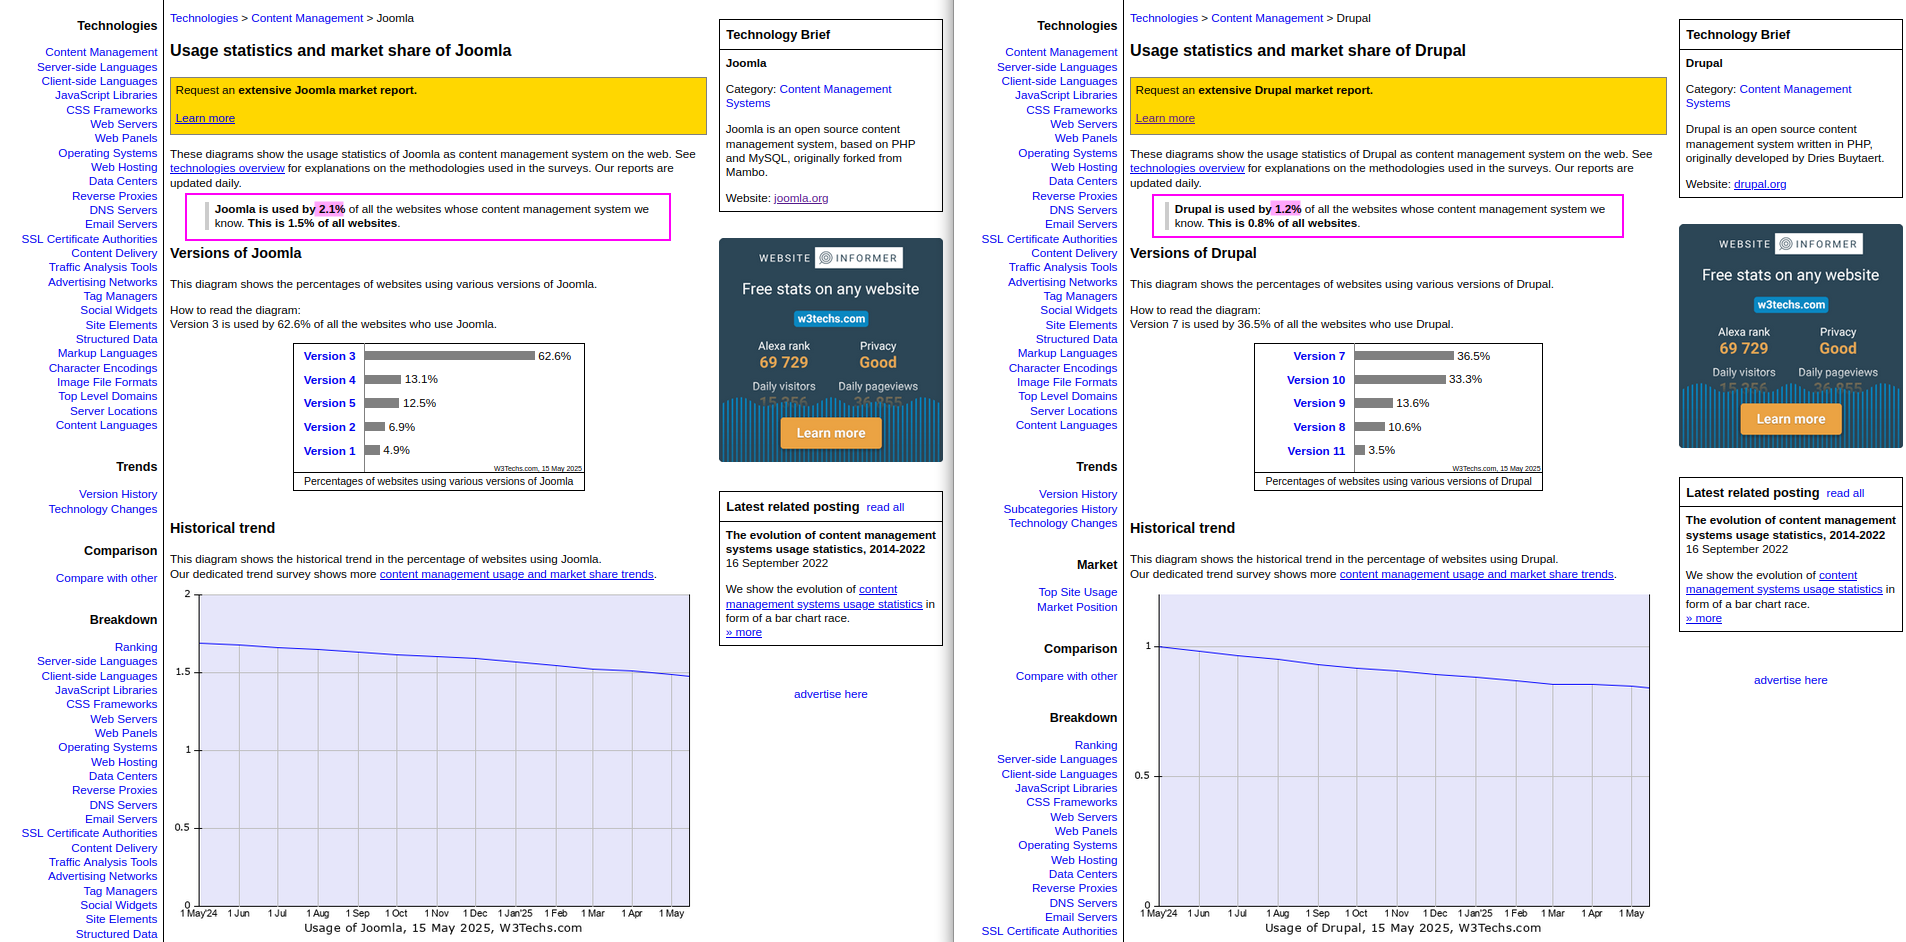
\includegraphics[width=0.85\textwidth]{images/usage-stats.png}
    \caption{Comparativa de cuota de mercado entre Joomla y Drupal según \href{https://w3techs.com/technologies/overview/content_management}{W3Techs}}
\end{figure}

\textgap

Joomla permite la creación de sitios web dinámicos y atractivos, con una amplia variedad de plantillas y extensiones disponibles totalmente gratuitas. Su interfaz intuitiva facilita la gestión de contenido, lo que es fundamental para mantener actualizada la información del negocio. En resumen, Joomla se presenta como una opción sólida y confiable para el desarrollo de la página web de una carnicería, ofreciendo las herramientas necesarias para crear una presencia en línea efectiva y profesional.

\newpage

\section{Instalación de Joomla}

Para esta práctica, al igual que con WordPress, se ha optado por instalar localmente Joomla utilizando Docker Compose, el archivo \texttt{docker-compose.yml} tiene los siguientes contenidos:


\begin{minted}[linenos, frame=single, fontsize=\small]{yaml}
version: '3.1'

services:
  db:
    image: mariadb:11.7.2-noble
    restart: no
    volumes:
      - ./db_data:/var/lib/mysql
    environment:
      - MARIADB_ROOT_PASSWORD=<MARIADB_ROOT_PASSWORD>
      - MARIADB_DATABASE=joomla_db
      - MARIADB_USER=joomlaAdmin
      - MARIADB_PASSWORD=<MARIADB_USER_PASSWORD>
    ports:
      - 3306:3306

  joomla:
    image: joomla:5.3.0-php8.3-apache
    restart: no
    volumes:
      - ./joomla_data:/var/www/html
    ports:
      - 80:80
    environment:
      - JOOMLA_DB_HOST=db:3306
      - JOOMLA_DB_USER=joomlaAdmin
      - JOOMLA_DB_PASSWORD=<MARIADB_USER_PASSWORD>
      - JOOMLA_DB_NAME=joomla_db
    depends_on:
      - db

  phpmyadmin:
    image: phpmyadmin:5.2.2-apache
    restart: no
    ports:
      - 8080:80
    environment:
      - PMA_HOST=db:3306
      - MYSQL_ROOT_PASSWORD=<MARIADB_ROOT_PASSWORD>
      - MYSQL_USER=joomlaAdmin
      - MYSQL_PASSWORD=<MARIADB_USER_PASSWORD>
    depends_on:
      - db
\end{minted}

\begin{figure}[H]
    \centering
    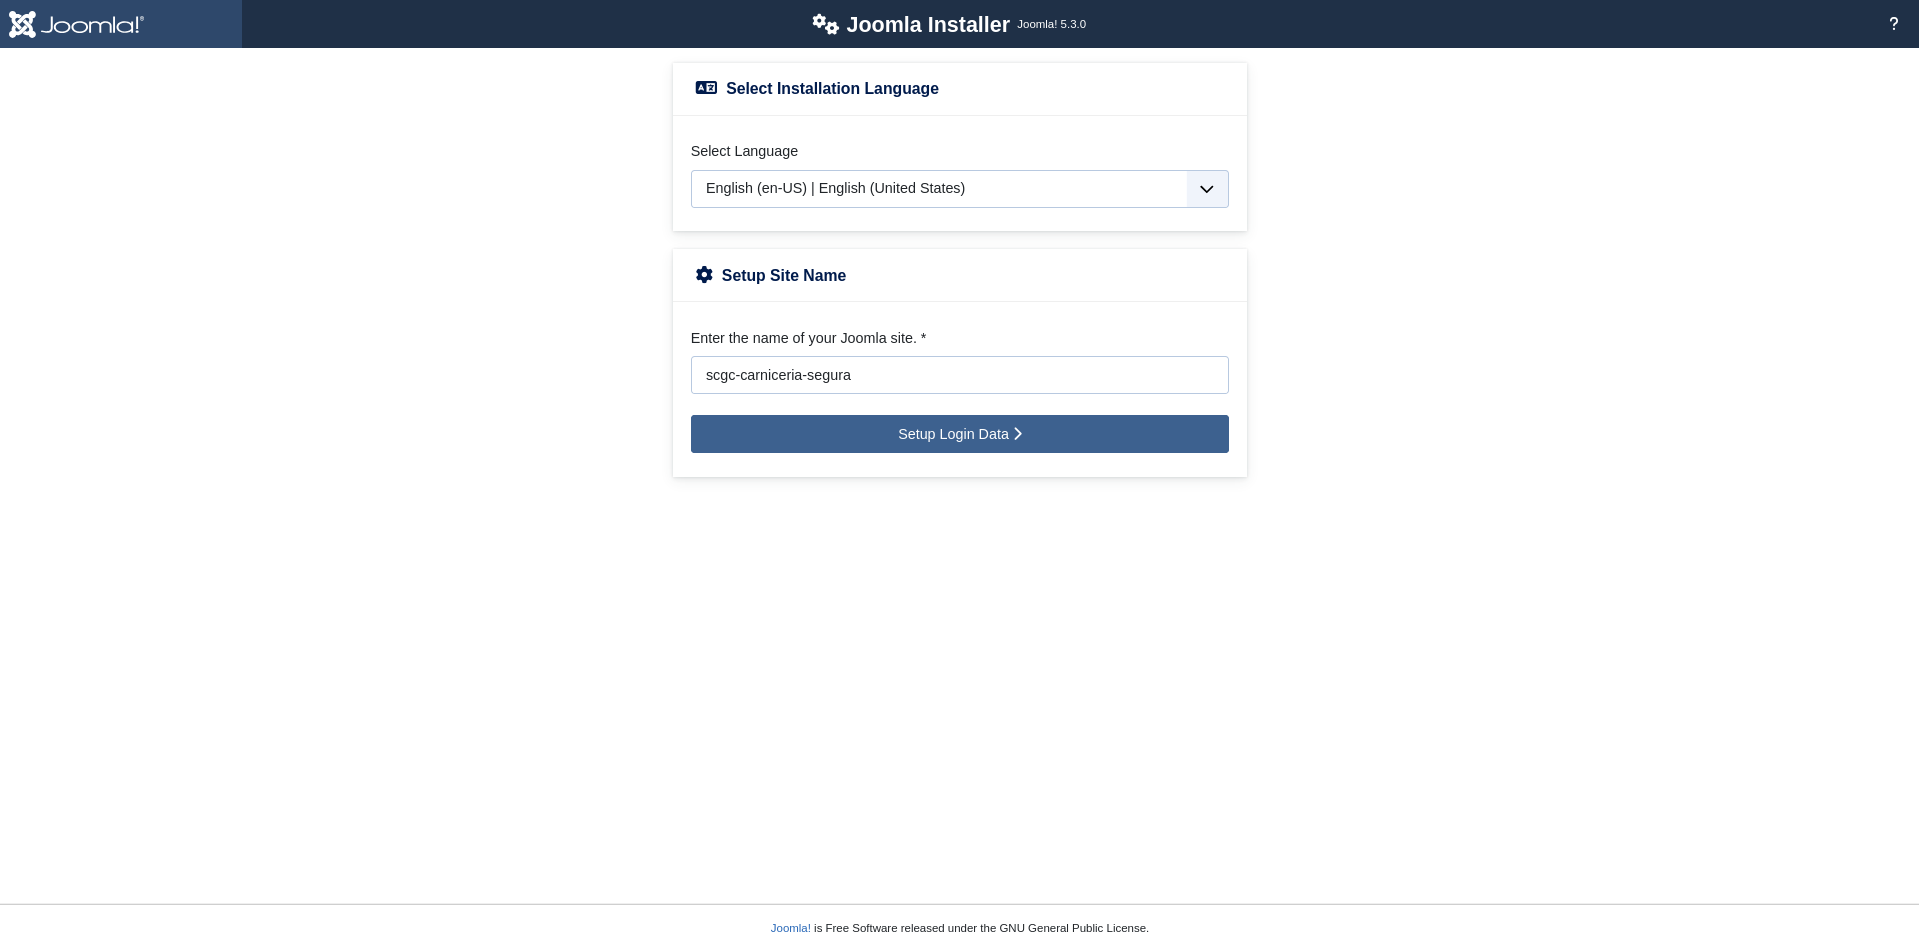
\includegraphics[width=0.85\textwidth]{images/install-1.png}
    \caption{Elección de lenguaje y nombre del sitio}
\end{figure}

\begin{figure}[H]
    \centering
    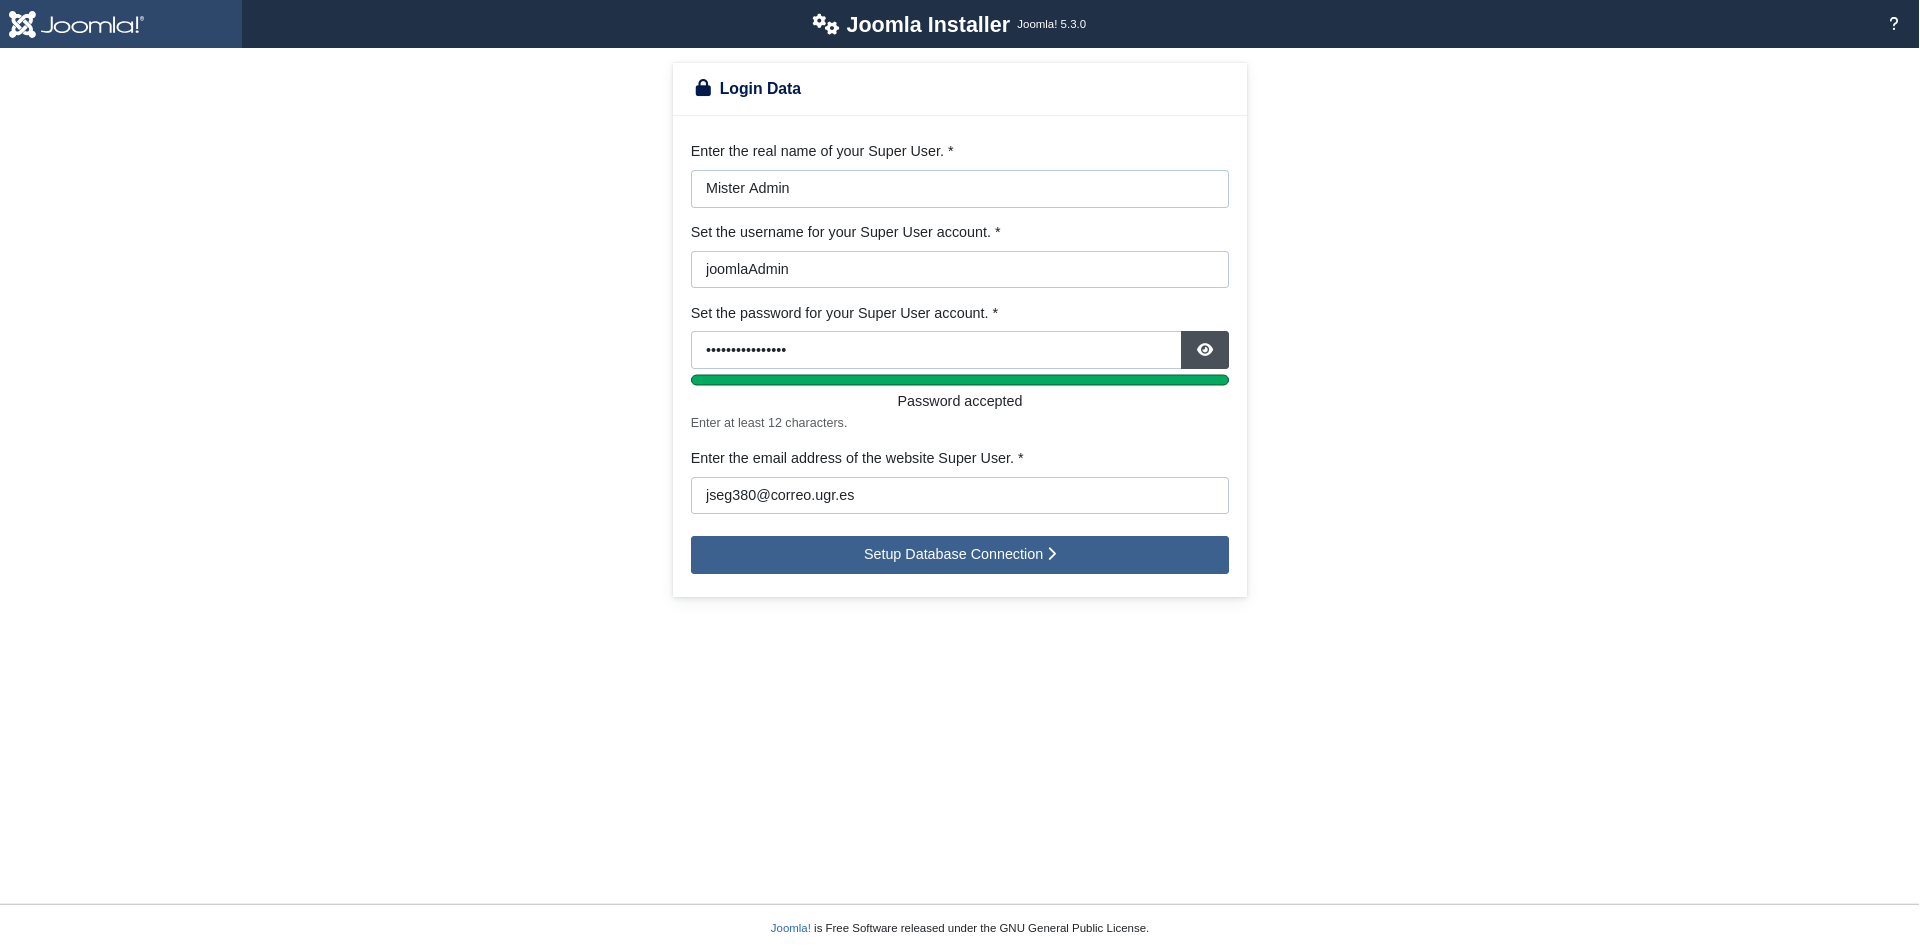
\includegraphics[width=0.85\textwidth]{images/install-2.png}
    \caption{Datos para login del administrador}
\end{figure}

\begin{figure}[H]
    \centering
    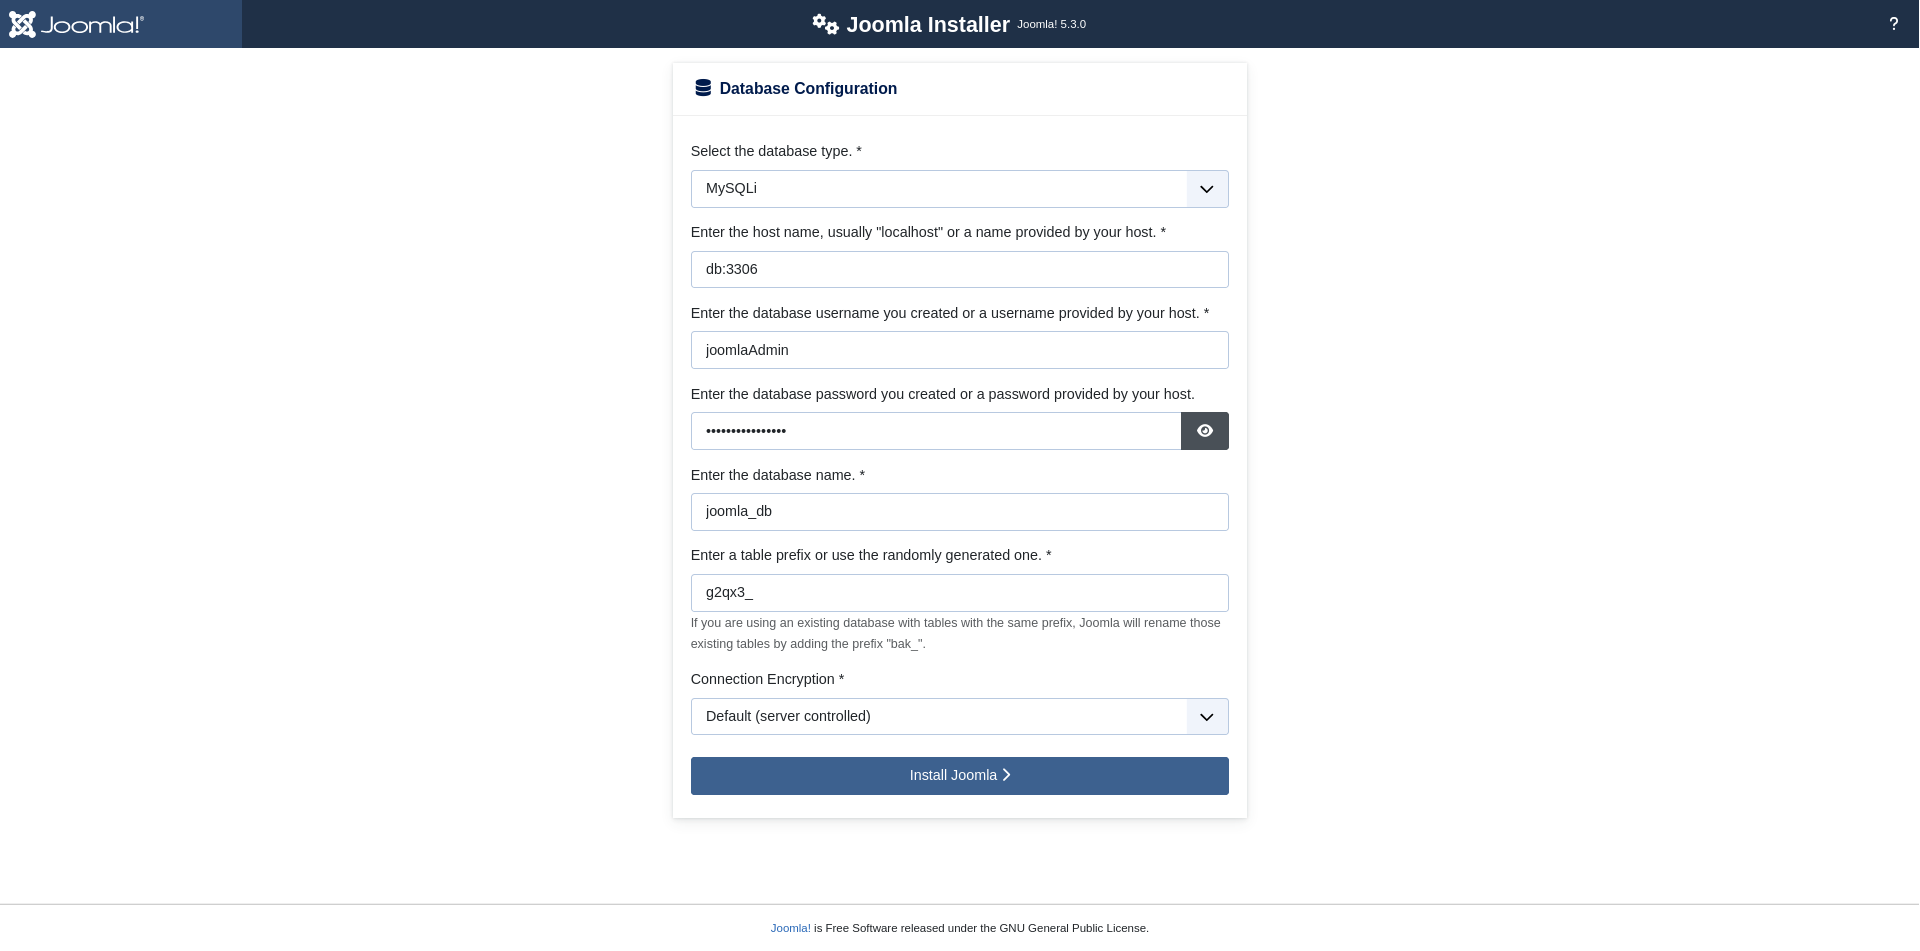
\includegraphics[width=0.85\textwidth]{images/install-3.png}
    \caption{Configuración de la base de datos}
\end{figure}

\begin{figure}[H]
    \centering
    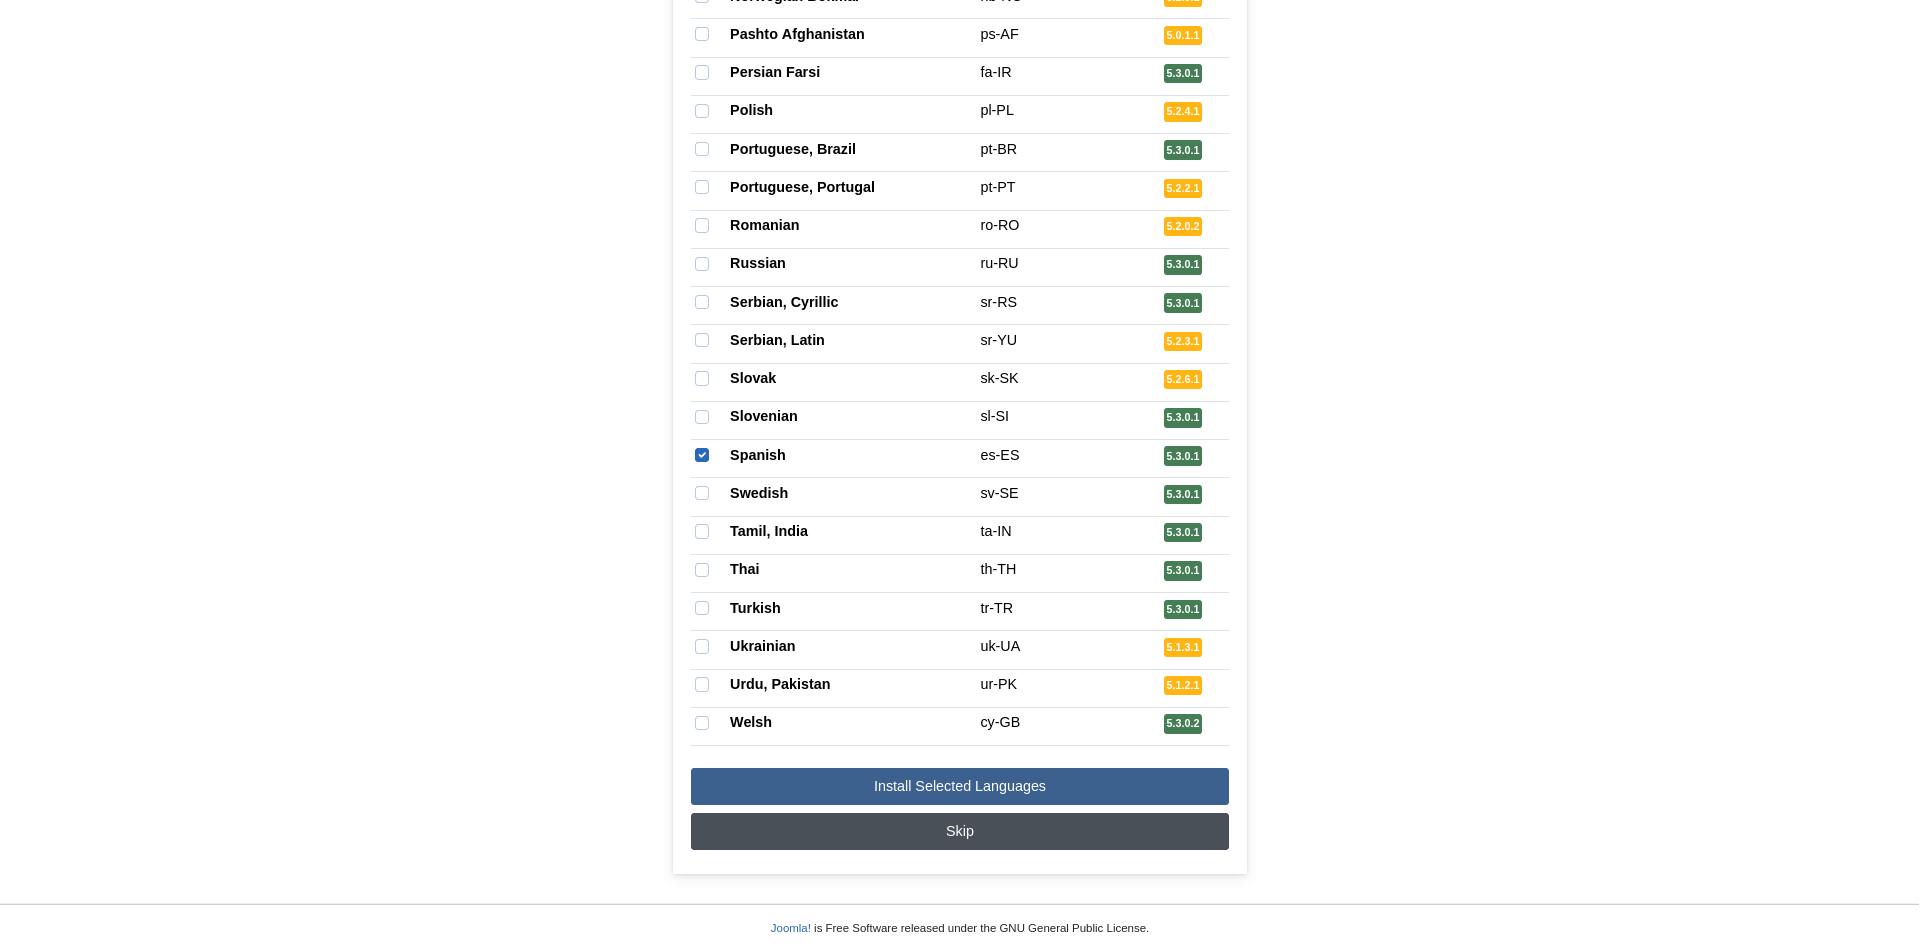
\includegraphics[width=0.8\textwidth]{images/install-4.png}
    \caption{Selección de lenguajes alternativos (inglés para administración y español para el usuario)}
\end{figure}

\begin{figure}[H]
    \centering
    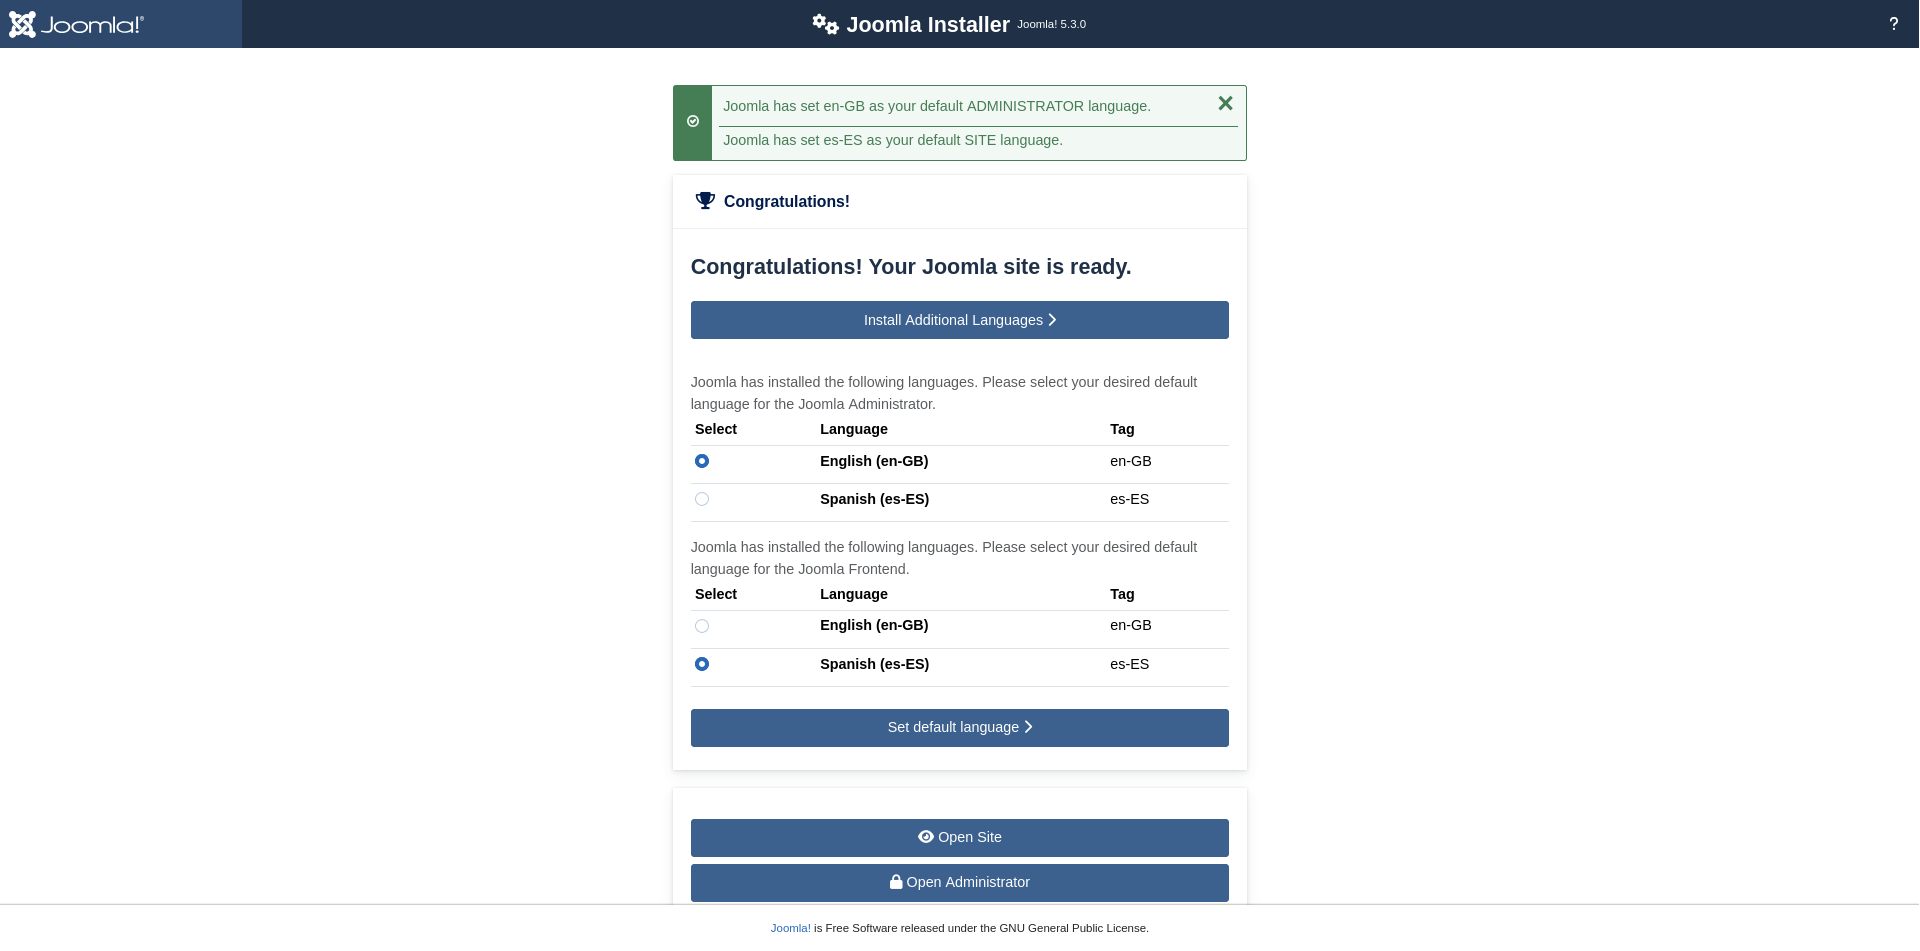
\includegraphics[width=0.8\textwidth]{images/install-5.png}
    \caption{Finalización de la instalación}
\end{figure}

\begin{figure}[H]
    \centering
    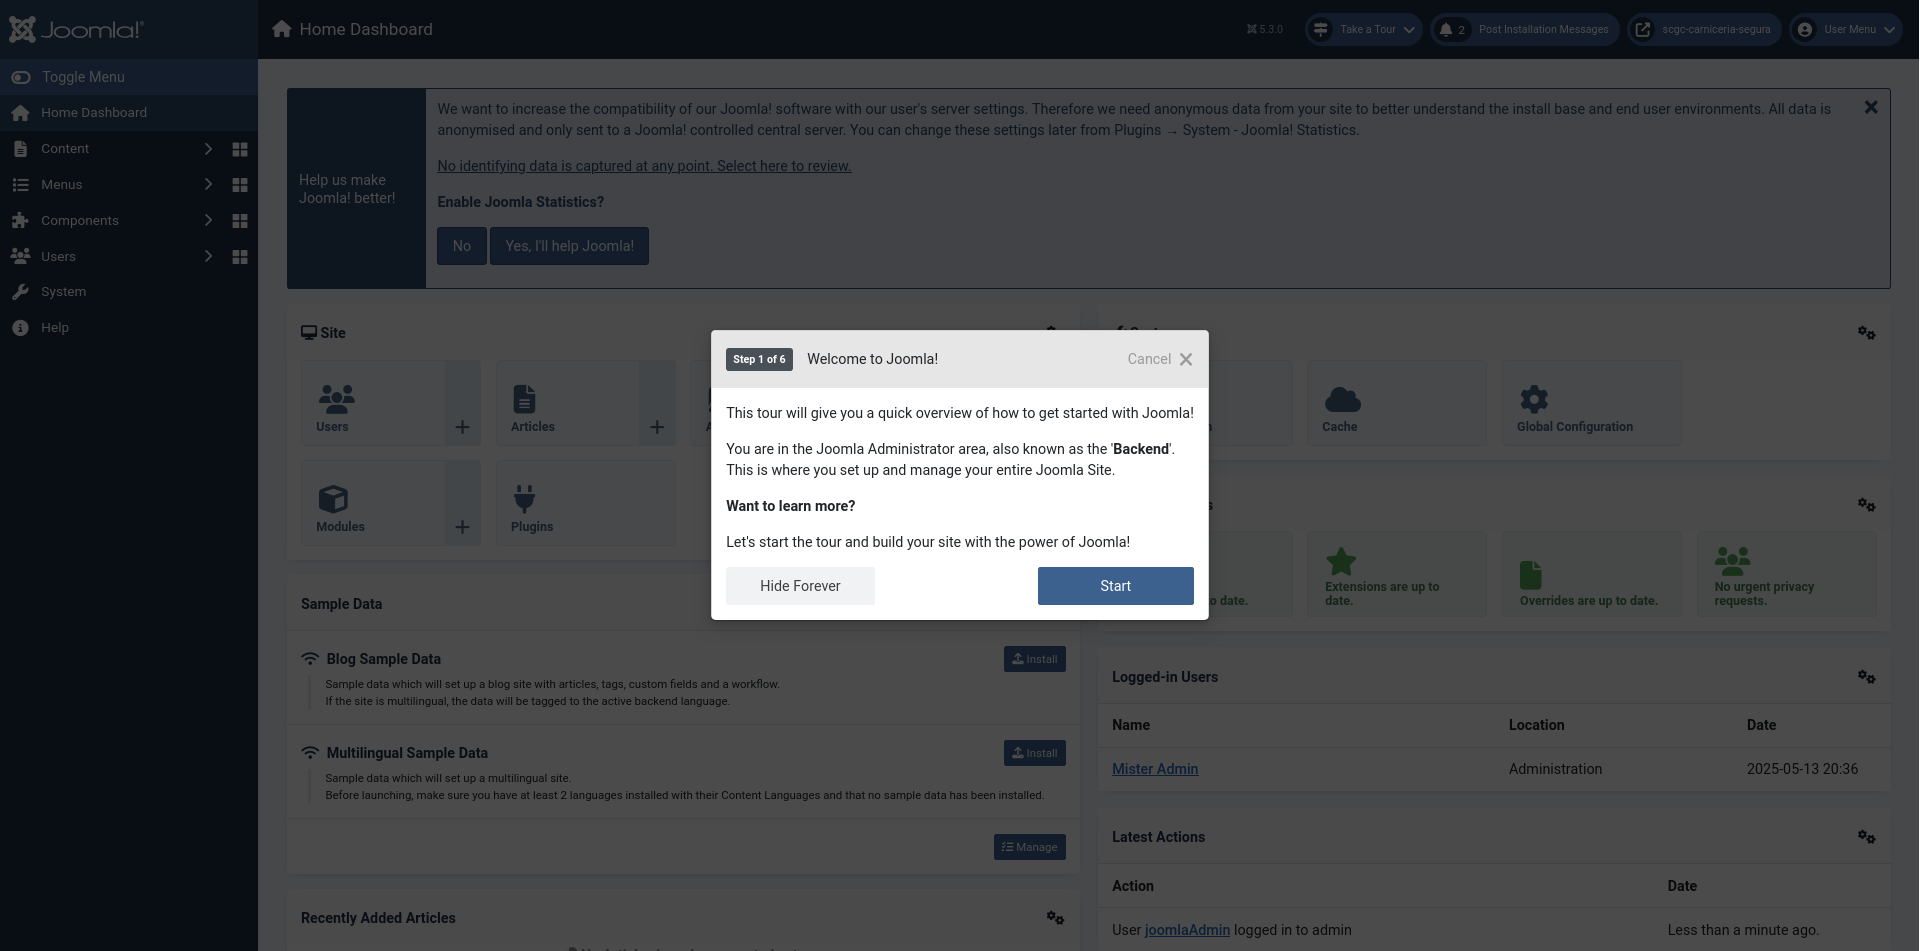
\includegraphics[width=0.8\textwidth]{images/install-6.png}
    \caption{Tour inicial de Joomla tras la instalación}
\end{figure}


\section{Selección e instalación de plantilla}

\subsection{Selección de plantilla}

Un breve análisis de las webs con plantillas para Joomla ha desvelado que gran cantidad de estas son de pago (Joomlart, Template Monster, Gavick, YooTheme) y aquellas que no lo son ofrecen una cantidad ínfima de plantillas gratuitas (\href{https://rockettheme.com/joomla/templates}{9 plantillas en RocketTheme (Filter by > Free) que están consideradas Legacy}, \href{https://www.themexpert.com/joomla-templates/tag/free}{2 plantillas en ThemExpert}). Por lo tanto, se ha optado por buscar plantillas gratuitas para Joomla en otras páginas.

\textgap

Tras una búsqueda de páginas que provean plantillas para Joomla gratuitas y actualizadas, la página \href{https://joomlead.com/joomla-template/}{Joomlead} ha sido la que más ha llamado la atención debido a su gran cantidad de plantillas gratuitas para Joomla que además de estar actualizadas, ofrecen un aspecto moderno y atractivo. Debido a la gran cantidad de plantillas que hay, en un primer análisis sobre el curso a tomar, se ha decidido optar por una plantilla con una estructura semejante a aquella de la usada para la página en WordPress y modificarla para corregir las variaciones que pueda tener.

\textgap

En concreto se ha optado por la plantilla \href{https://joomlead.com/joomla-template/bruno/}{Bruno}, plantilla para Joomla 4.x y 5.x, que hace uso del framework Gantry y que se actualizó por última vez (a la fecha de redacción de este documento) el 6 de mayo de 2025. Esta plantilla es completamente gratuita y se puede descargar desde la página de Joomlead.

\begin{figure}[H]
    \centering
    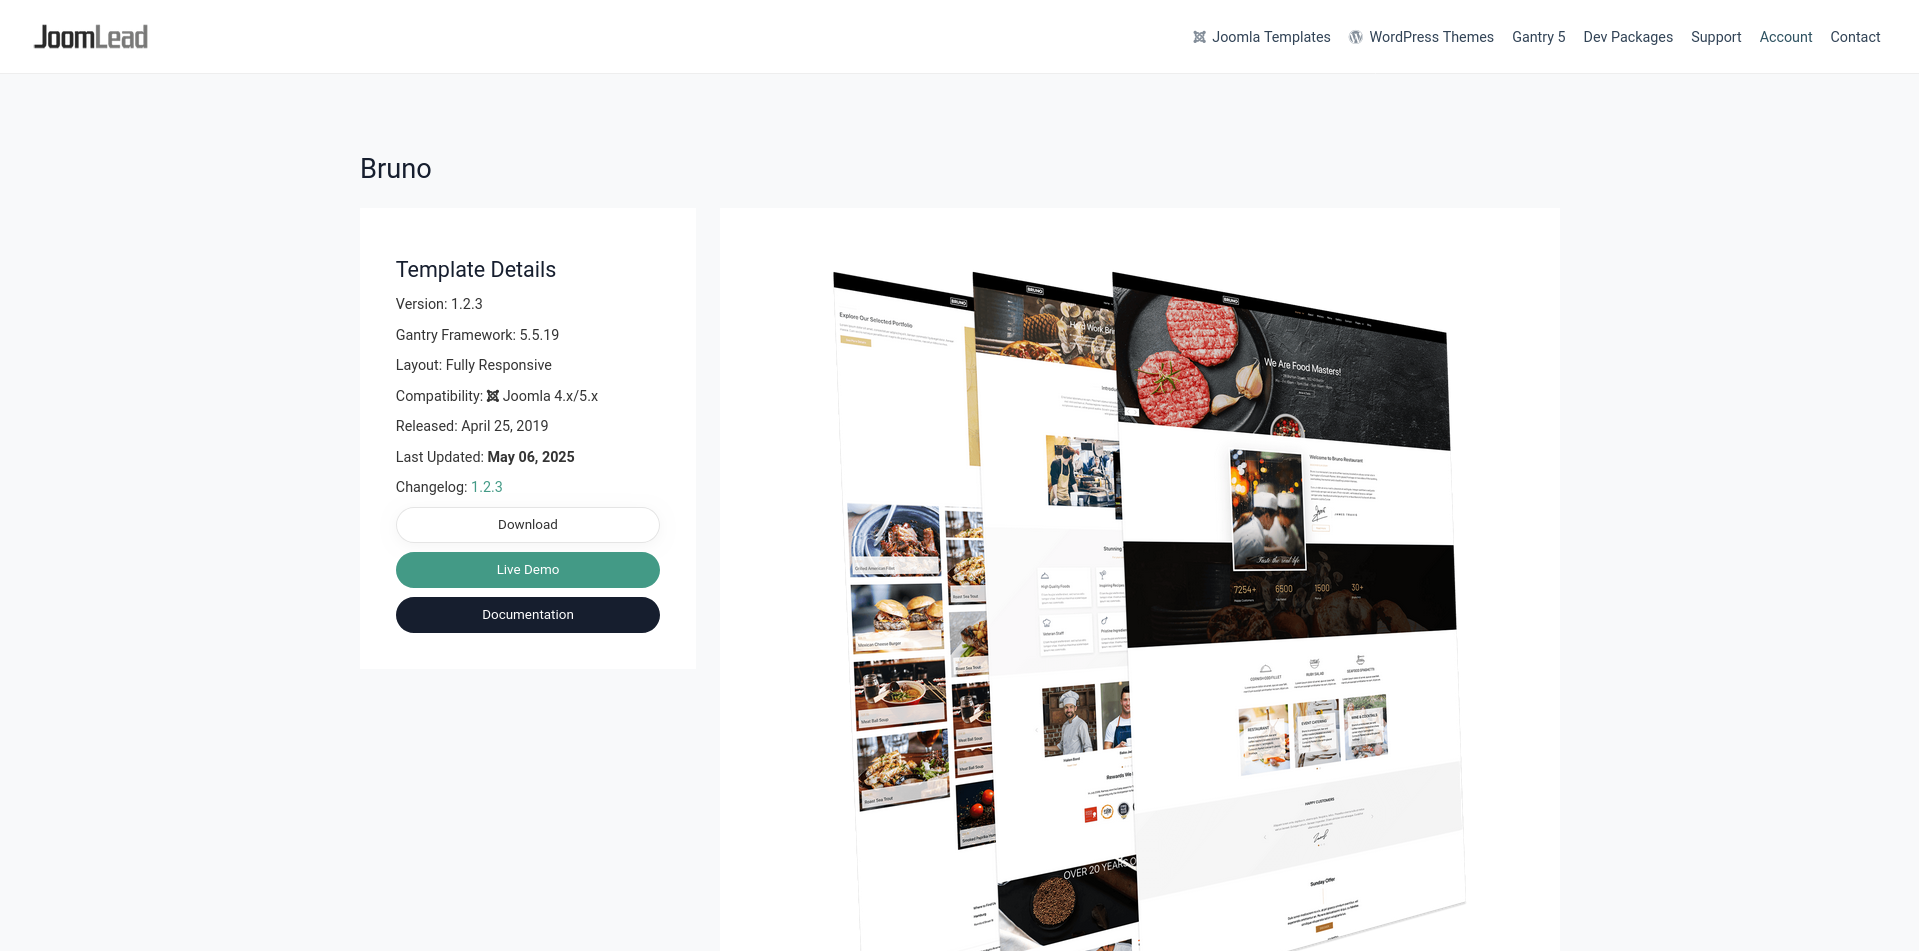
\includegraphics[width=0.85\textwidth]{images/template-details.png}
    \caption{Plantilla Bruno en Joomlead}
\end{figure}

\subsection{Instalación de la plantilla}

Como se ha mencionado anteriormente, la plantilla seleccionada hace uso del framework Gantry, por lo que es necesario instalarlo antes de poder usar la plantilla. Para ello, se ha seguido la \href{https://joomlead.com/documentation/bruno-documentation/}{guía de instalación propia a la plantilla seleccionada}, donde se explica cómo instalar Gantry y hacer uso de la plantilla en sí. Una forma fácil de obtener el framework es haciendo uso del instalador de plugins que Joomla proporciona, permite instalar plugins locales y, al igual que WordPress, ofrece un instalador de plugins online.

\begin{figure}[H]
    \centering
    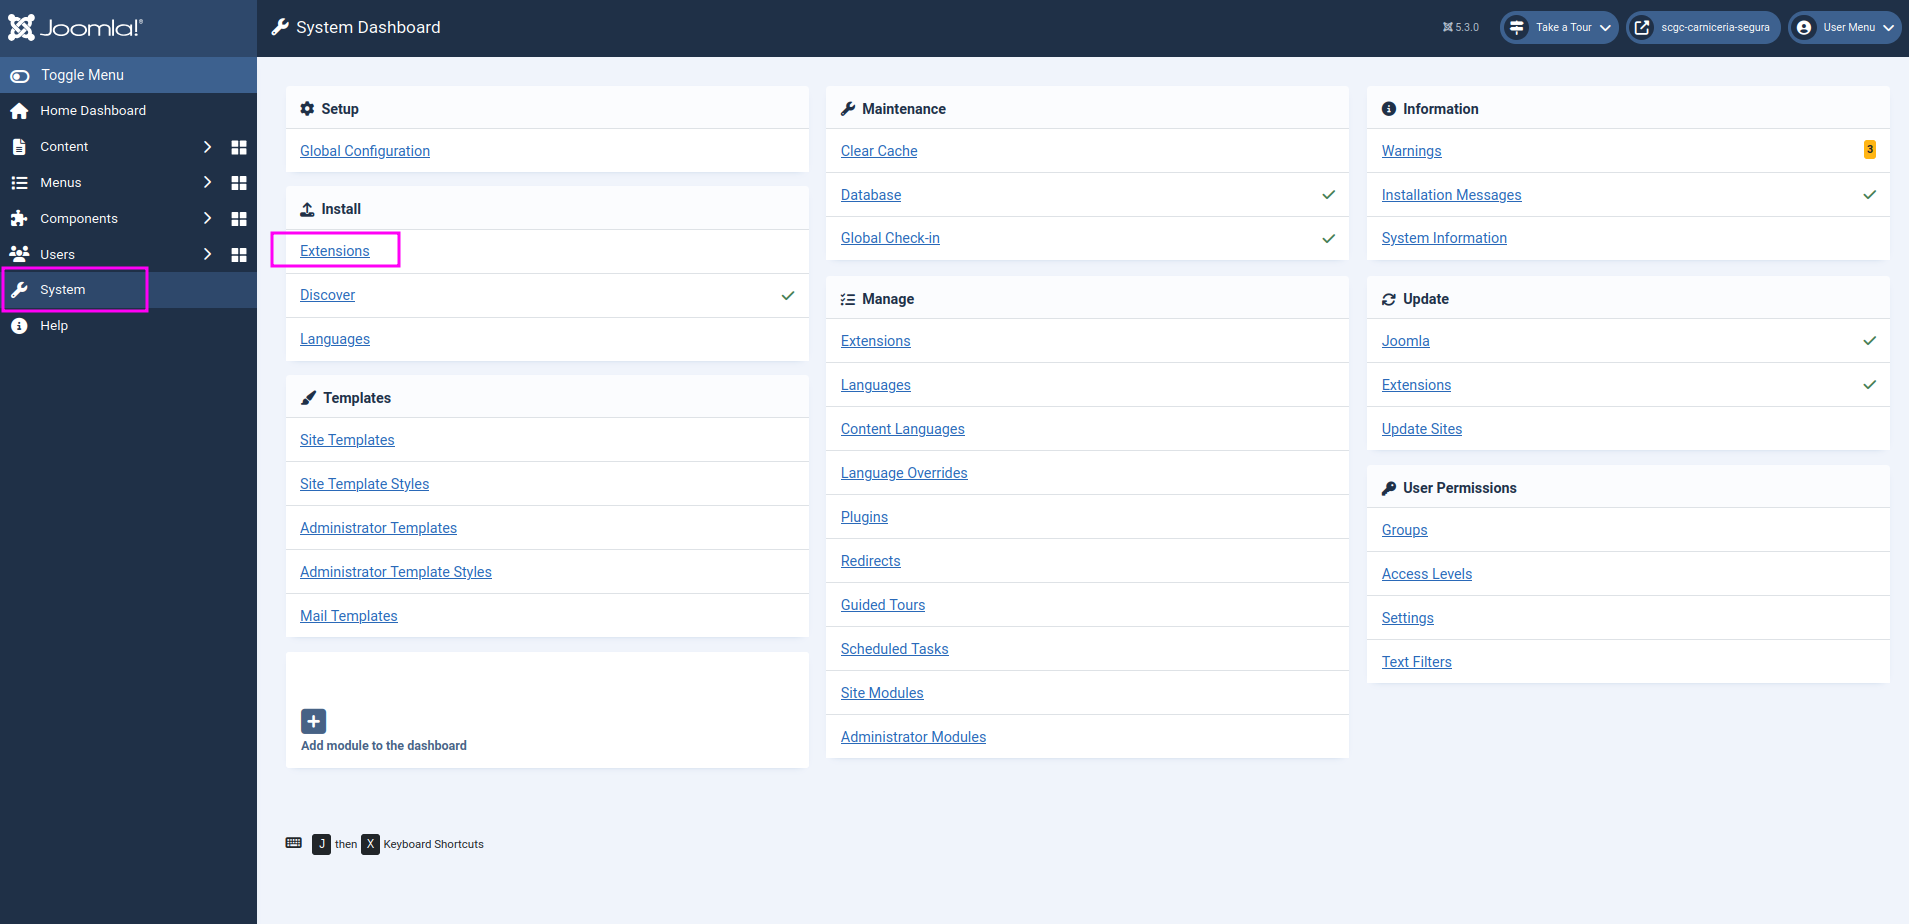
\includegraphics[width=0.8\textwidth]{images/gantry5-install-1.png}
    \caption{Acceso al instalador de extensiones}
\end{figure}

\begin{figure}[H]
    \centering
    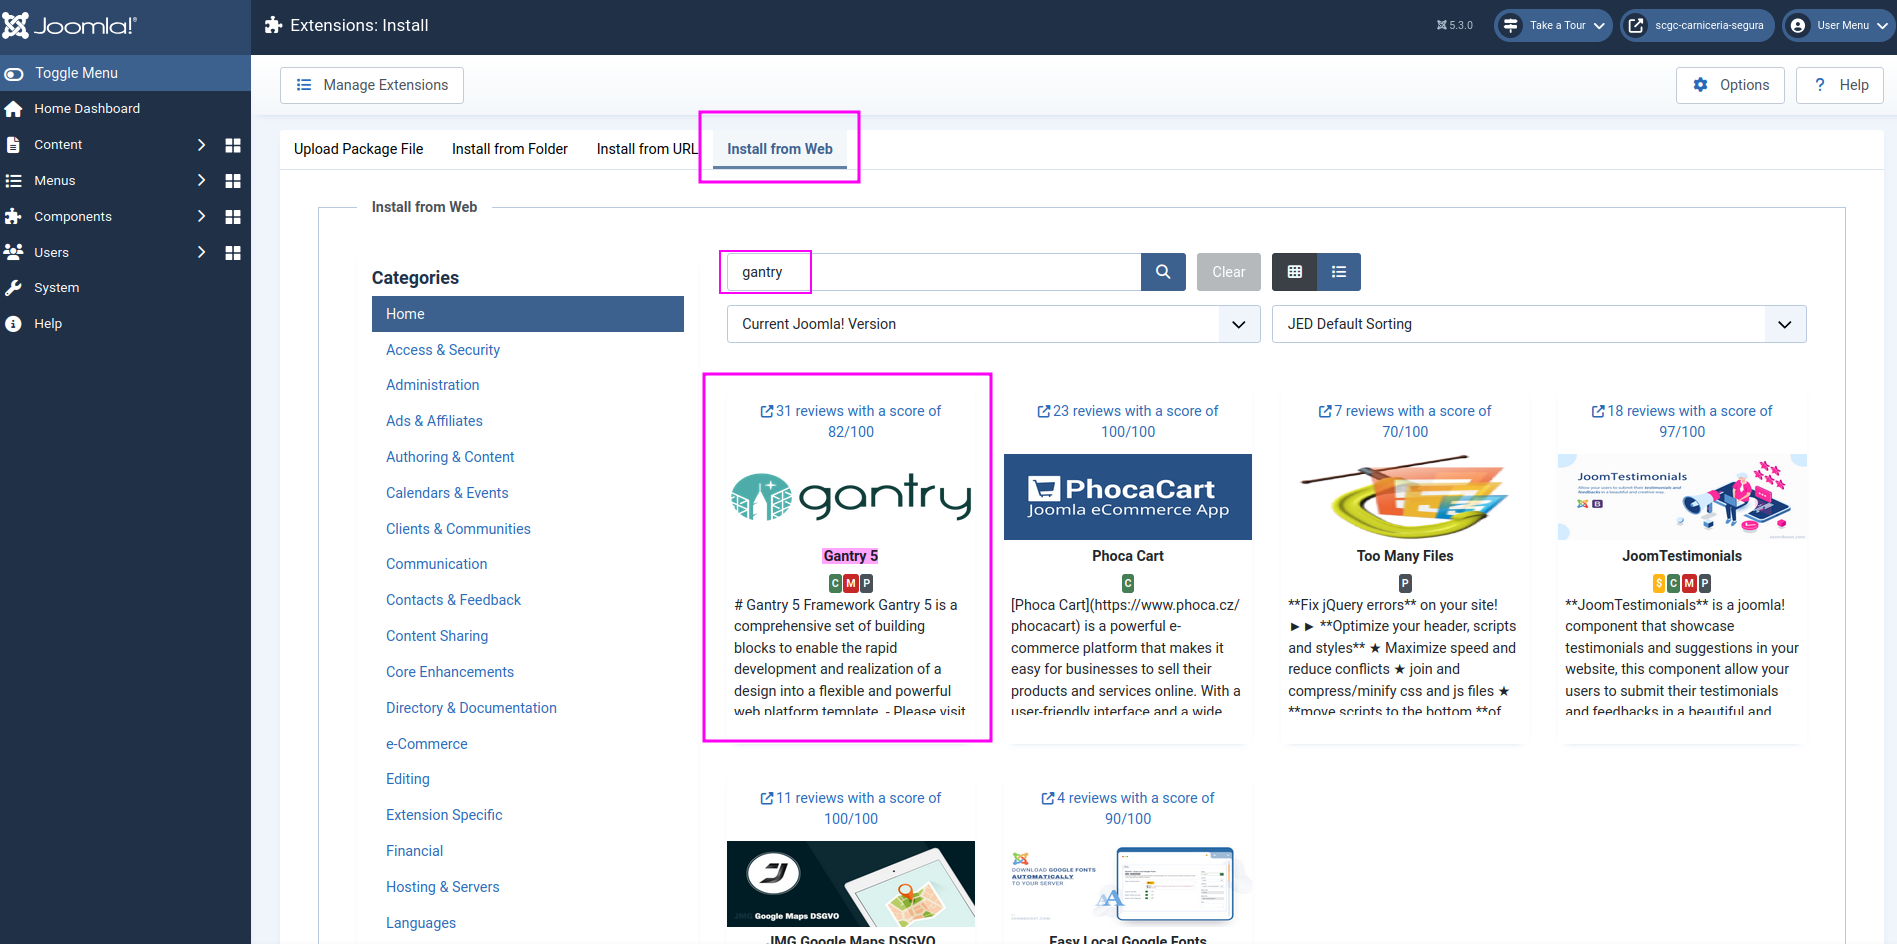
\includegraphics[width=0.8\textwidth]{images/gantry5-install-2.png}
    \caption{Búsqueda y selección de Gantry 5}
\end{figure}

\begin{figure}[H]
    \centering
    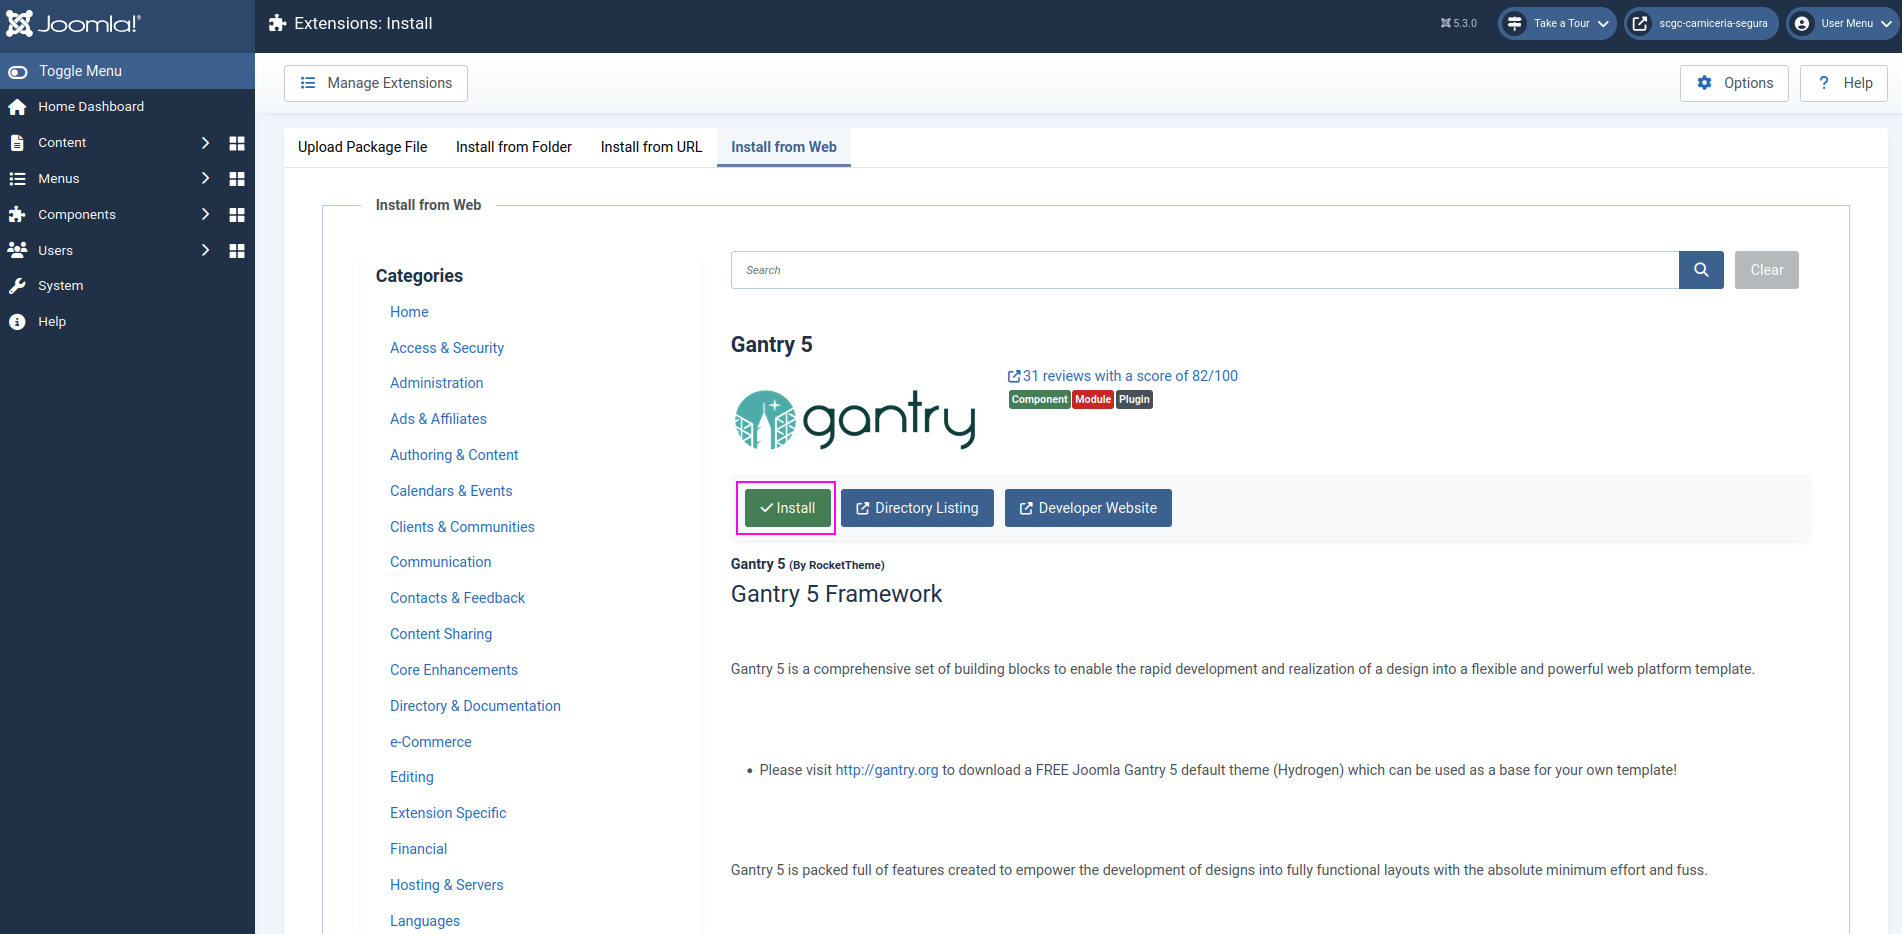
\includegraphics[width=0.8\textwidth]{images/gantry5-install-3.png}
    \caption{Instalación de Gantry 5}
\end{figure}


\section{Configuración de la plantilla}

Una vez instalada la plantilla, se ha procedido a configurarla para que se asemeje lo máximo posible a la plantilla de WordPress. Para ello, se ha seguido la \href{https://joomlead.com/documentation/bruno-documentation/}{guía de configuración de la plantilla Bruno} y tras una fase inicial de familiarización con el editor, se ha procedido a la edición de la plantilla. En las siguientes imágenes se puede ver el proceso de edición de la misma.

\begin{figure}[H]
    \centering
    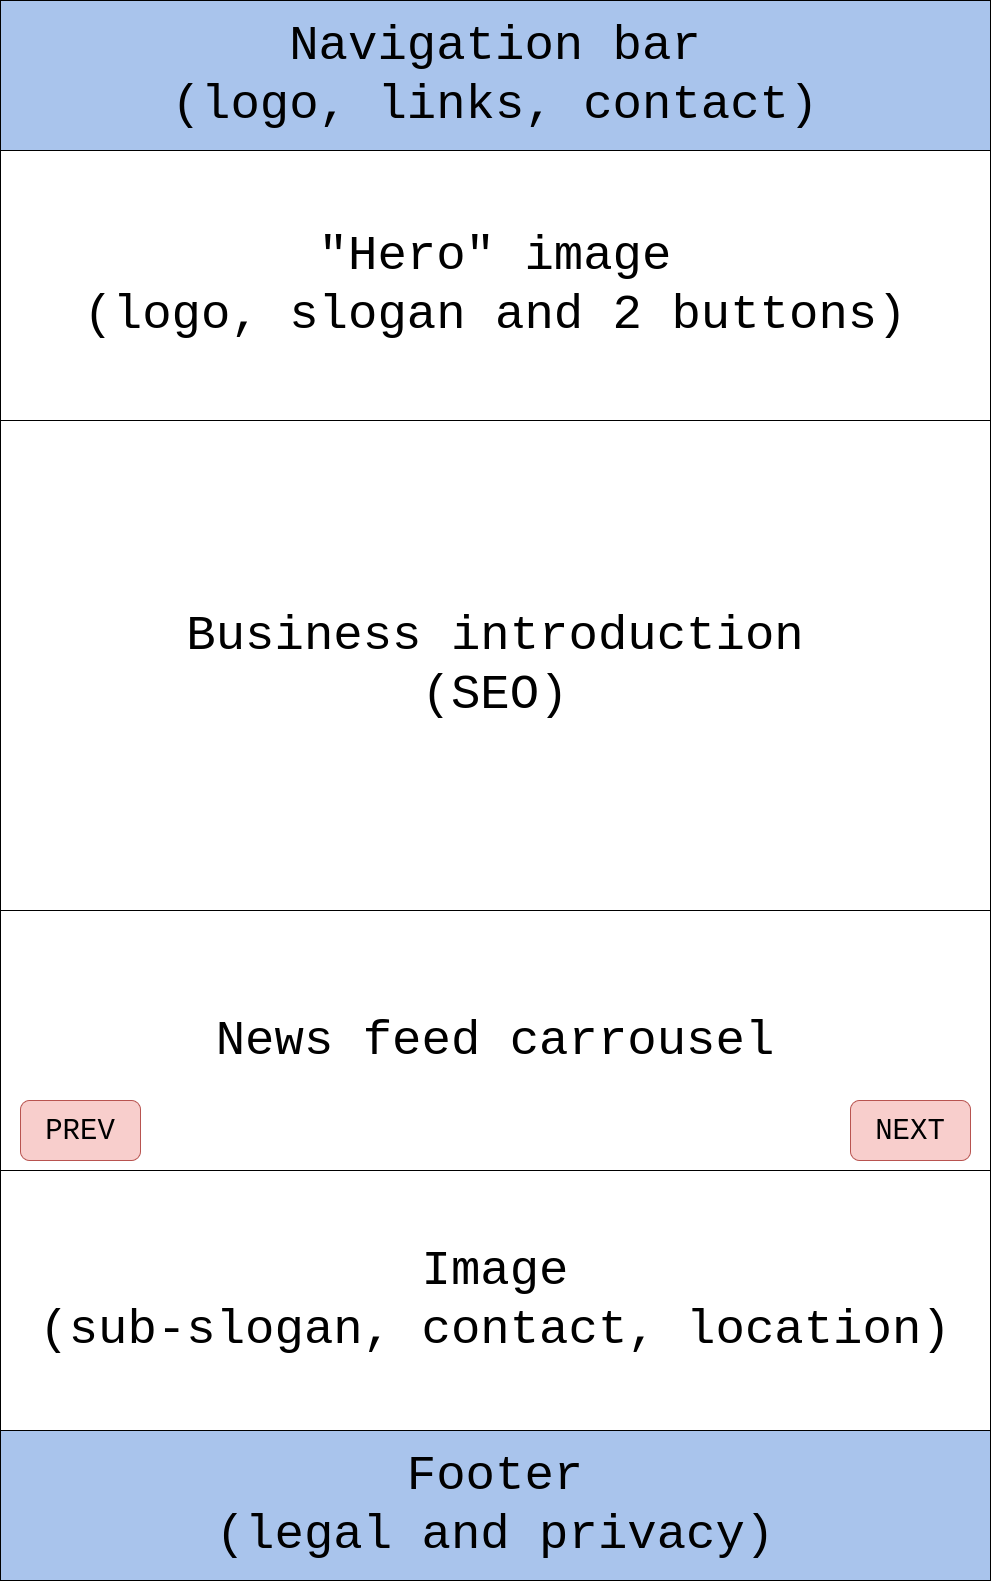
\includegraphics[width=0.65\textwidth]{images/landing-page-template.png}
    \captionsetup{width=0.6\textwidth}
    \caption{Landing page template (imagen para cuadrar el resto de imágenes de la sección)}
\end{figure}

\begin{figure}[H]
    \centering
    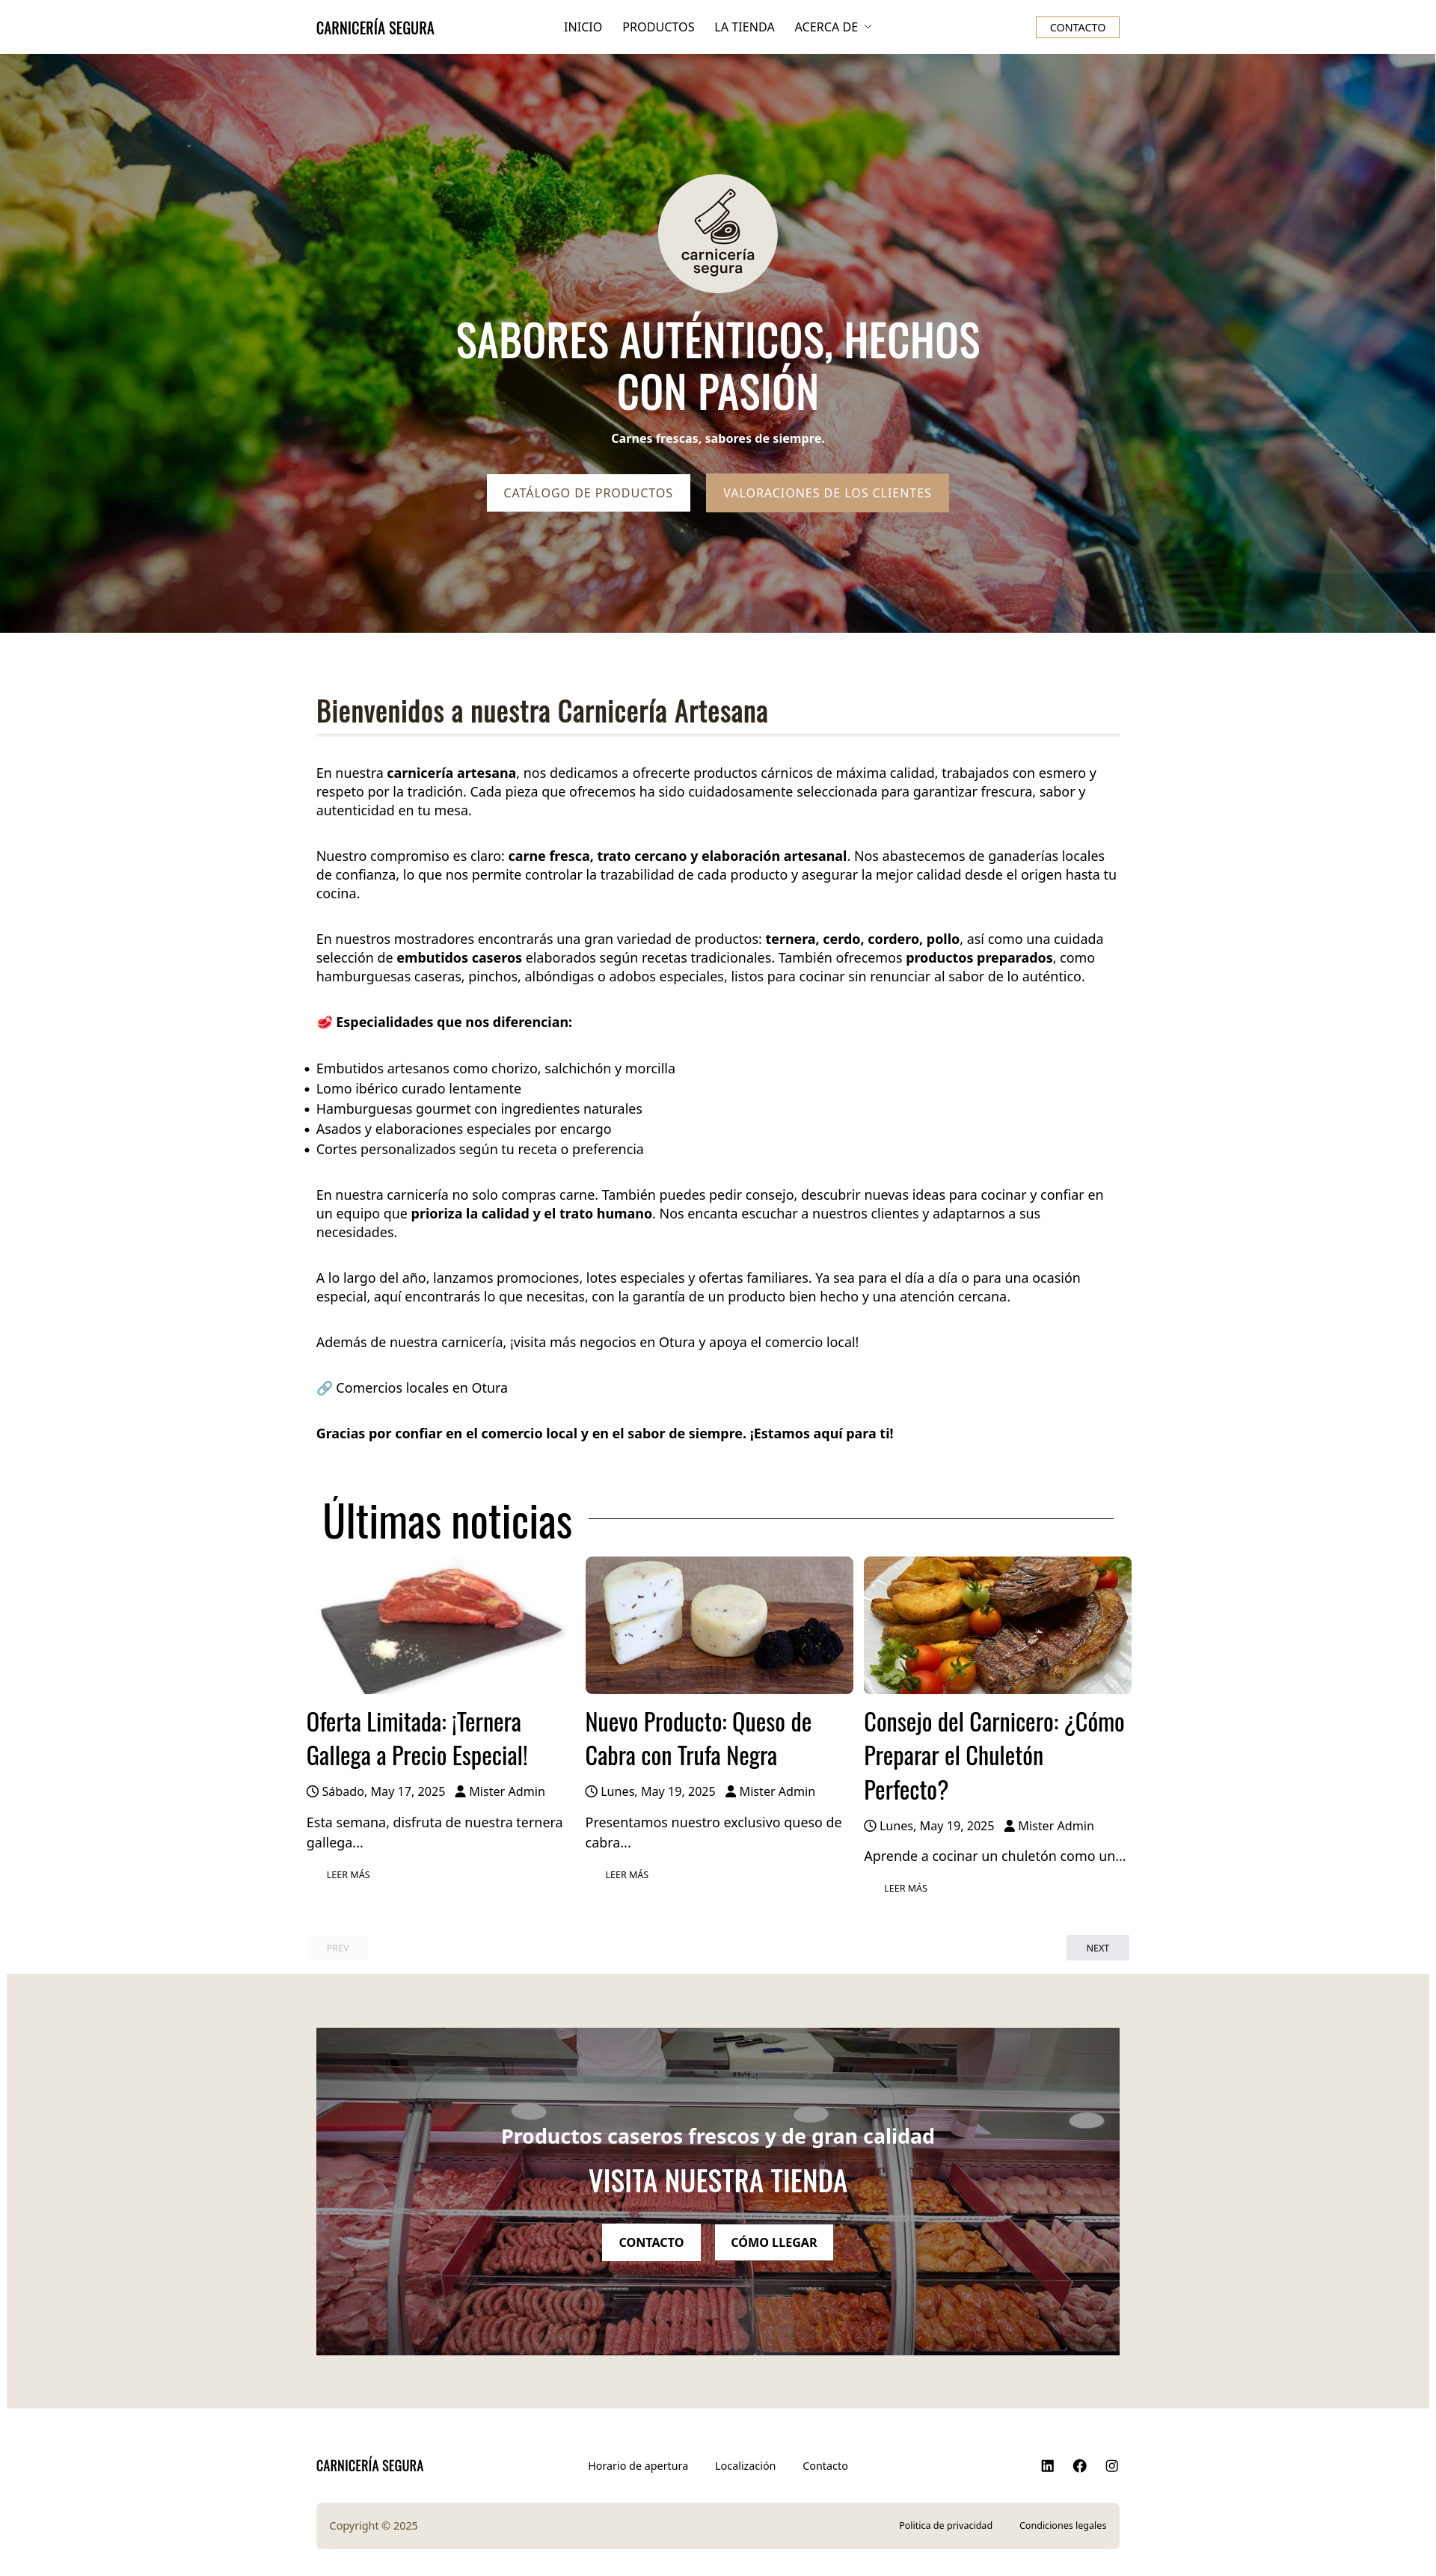
\includegraphics[width=0.85\textwidth]{images/template-1.png}
    \caption{Landing page}
\end{figure}

\begin{figure}[H]
    \centering
    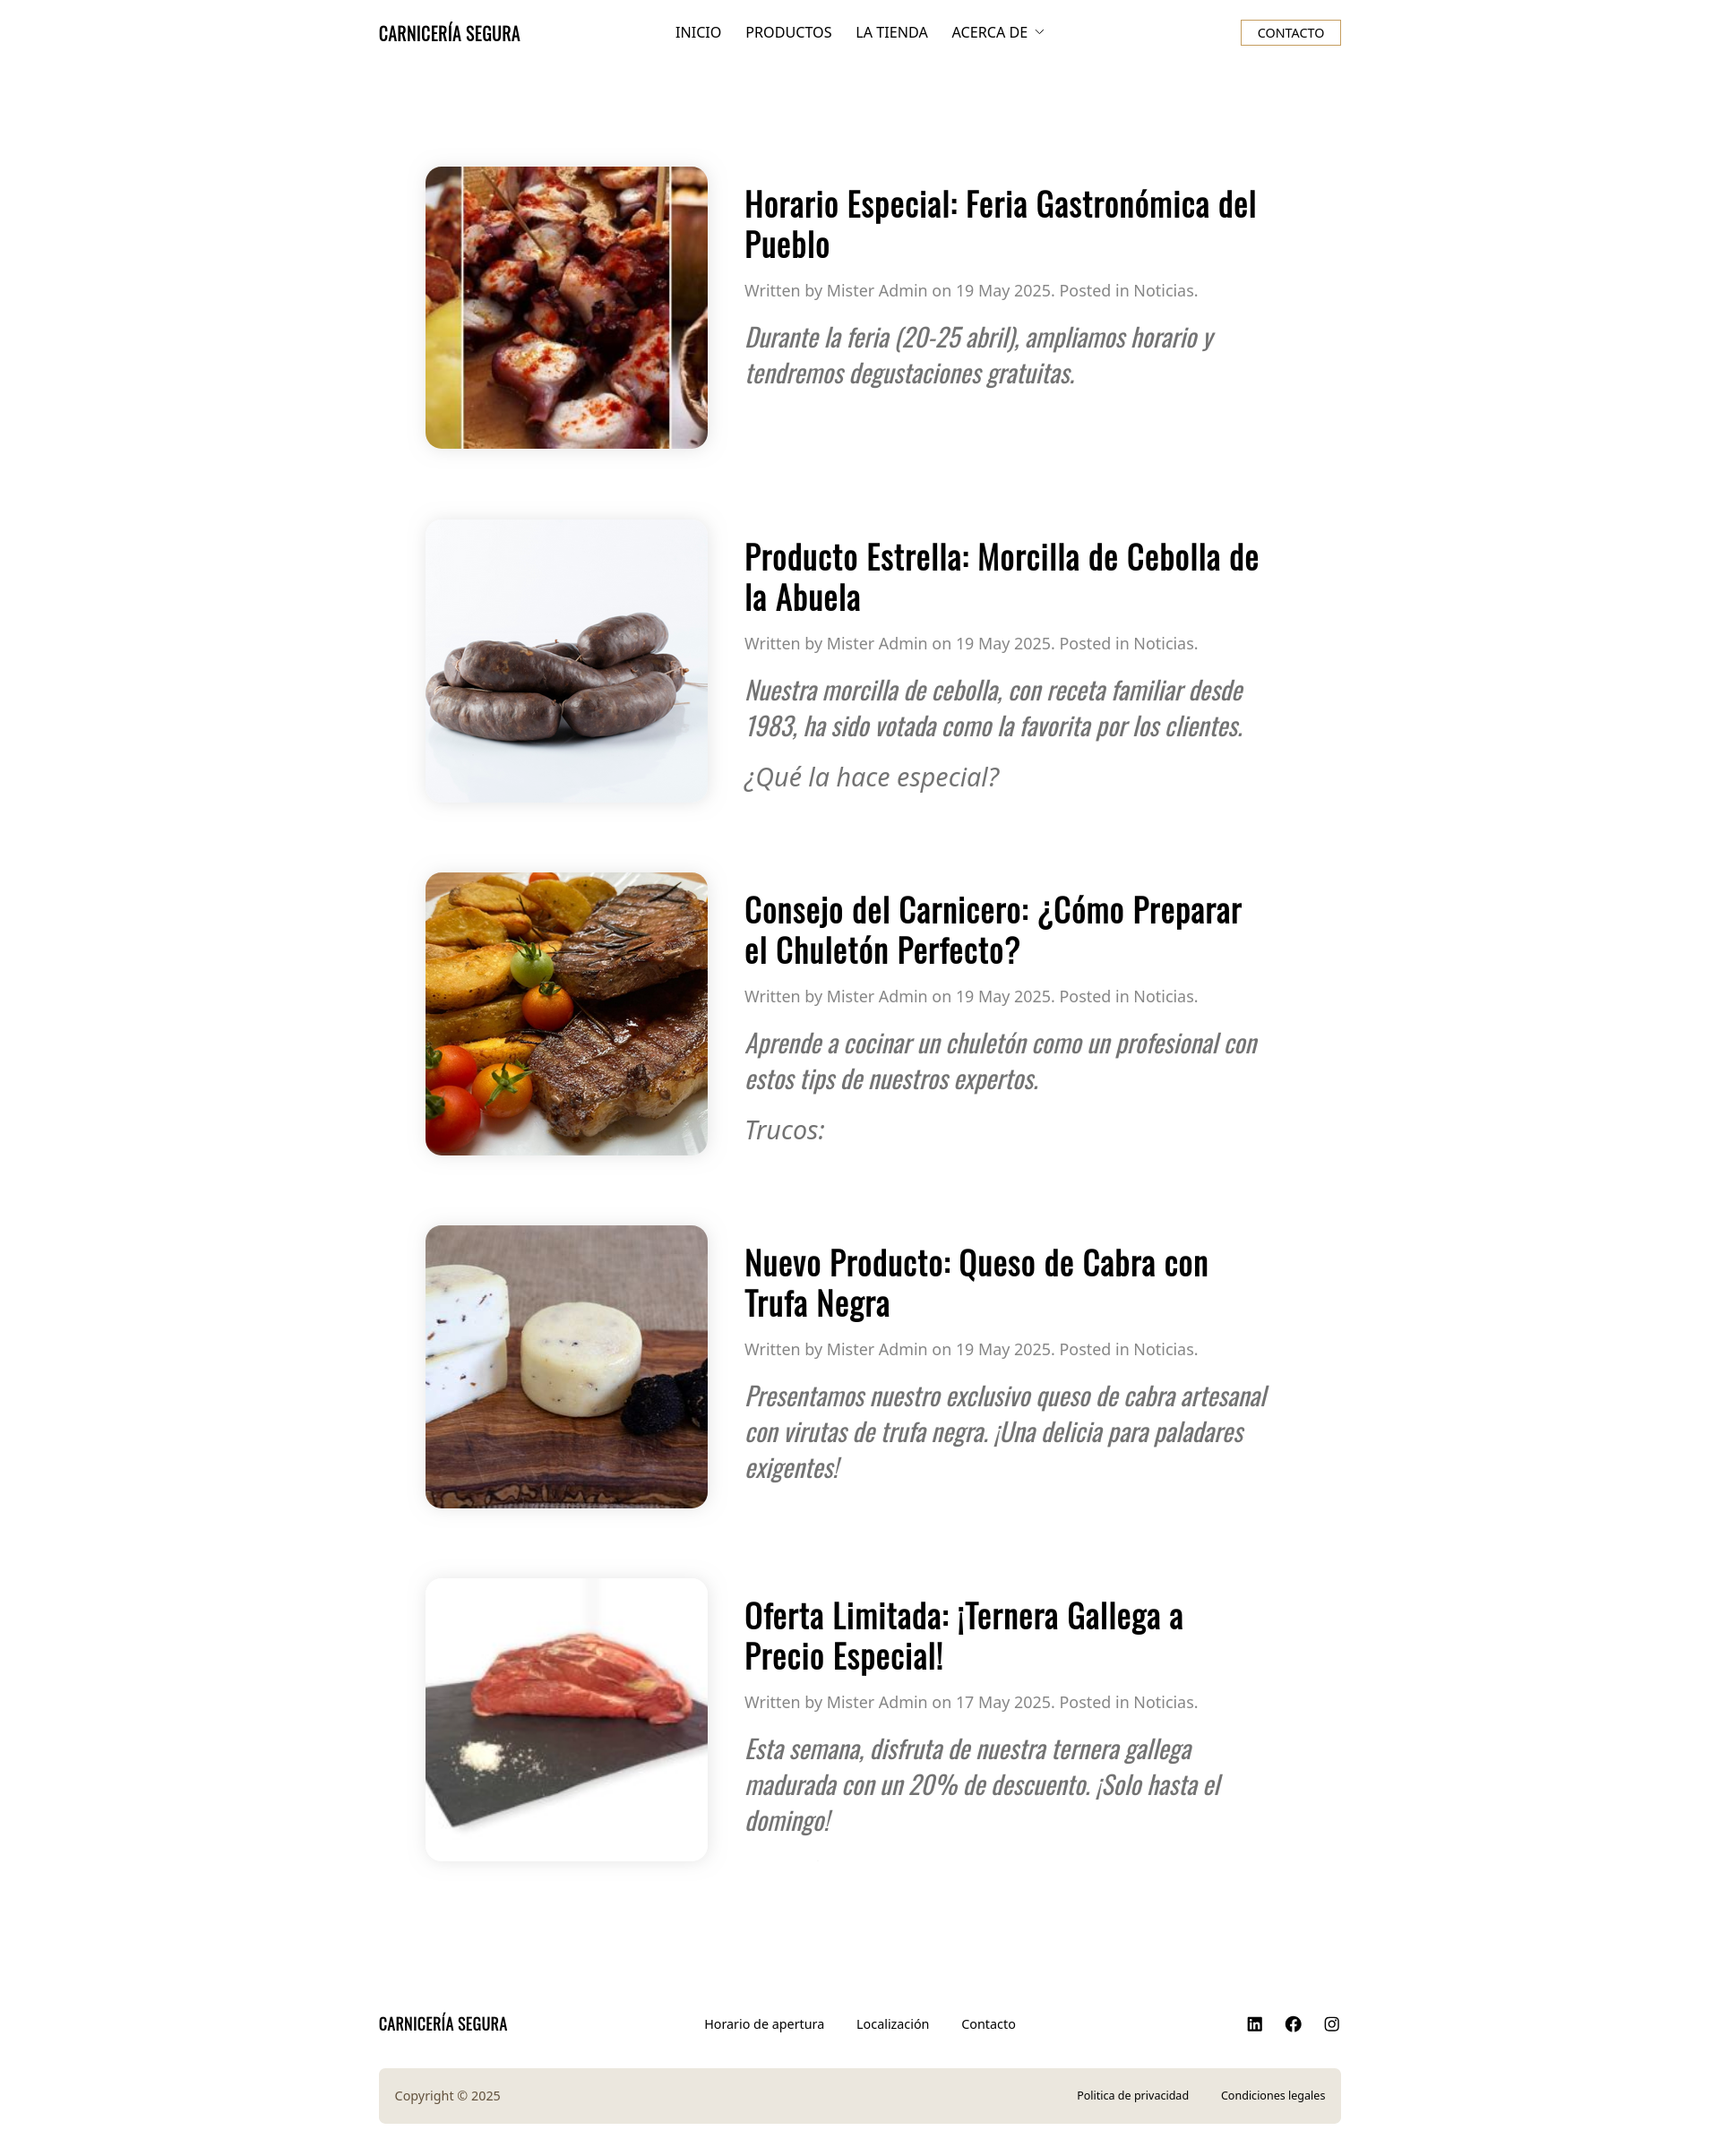
\includegraphics[width=1\textwidth]{images/template-2.png}
    \caption{Página con todas las noticias}
\end{figure}

\begin{figure}[H]
    \centering
    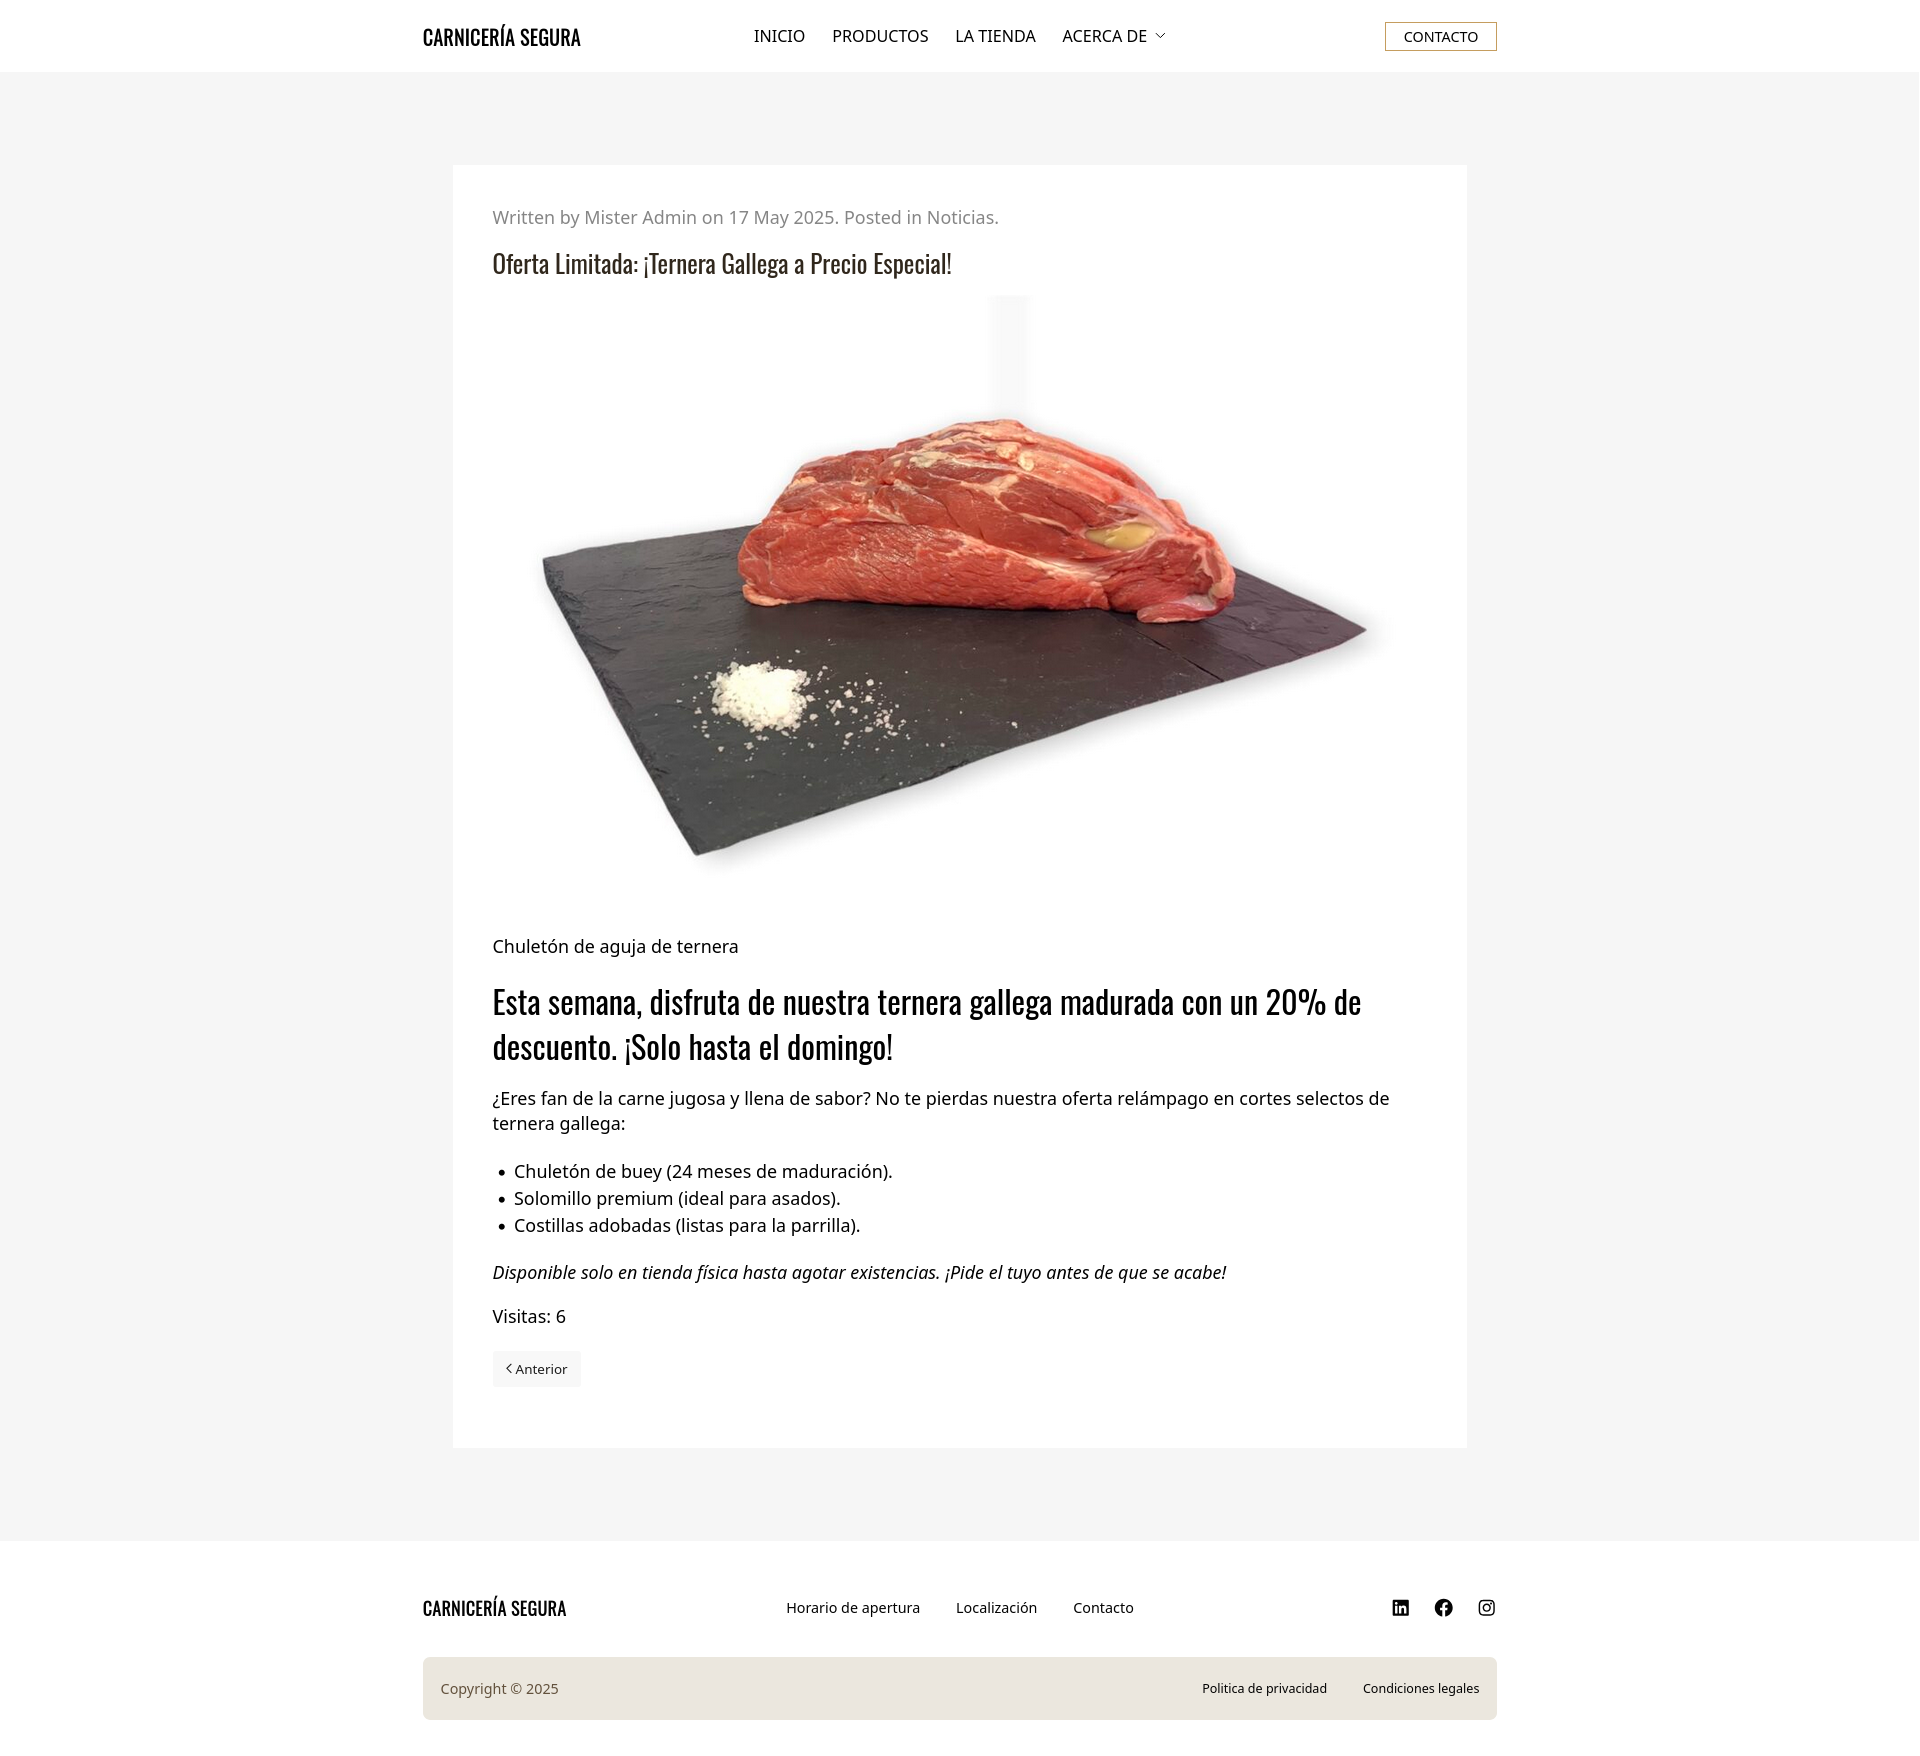
\includegraphics[width=1\textwidth]{images/template-3.png}
    \caption{Noticia}
\end{figure}

\begin{figure}[H]
    \centering
    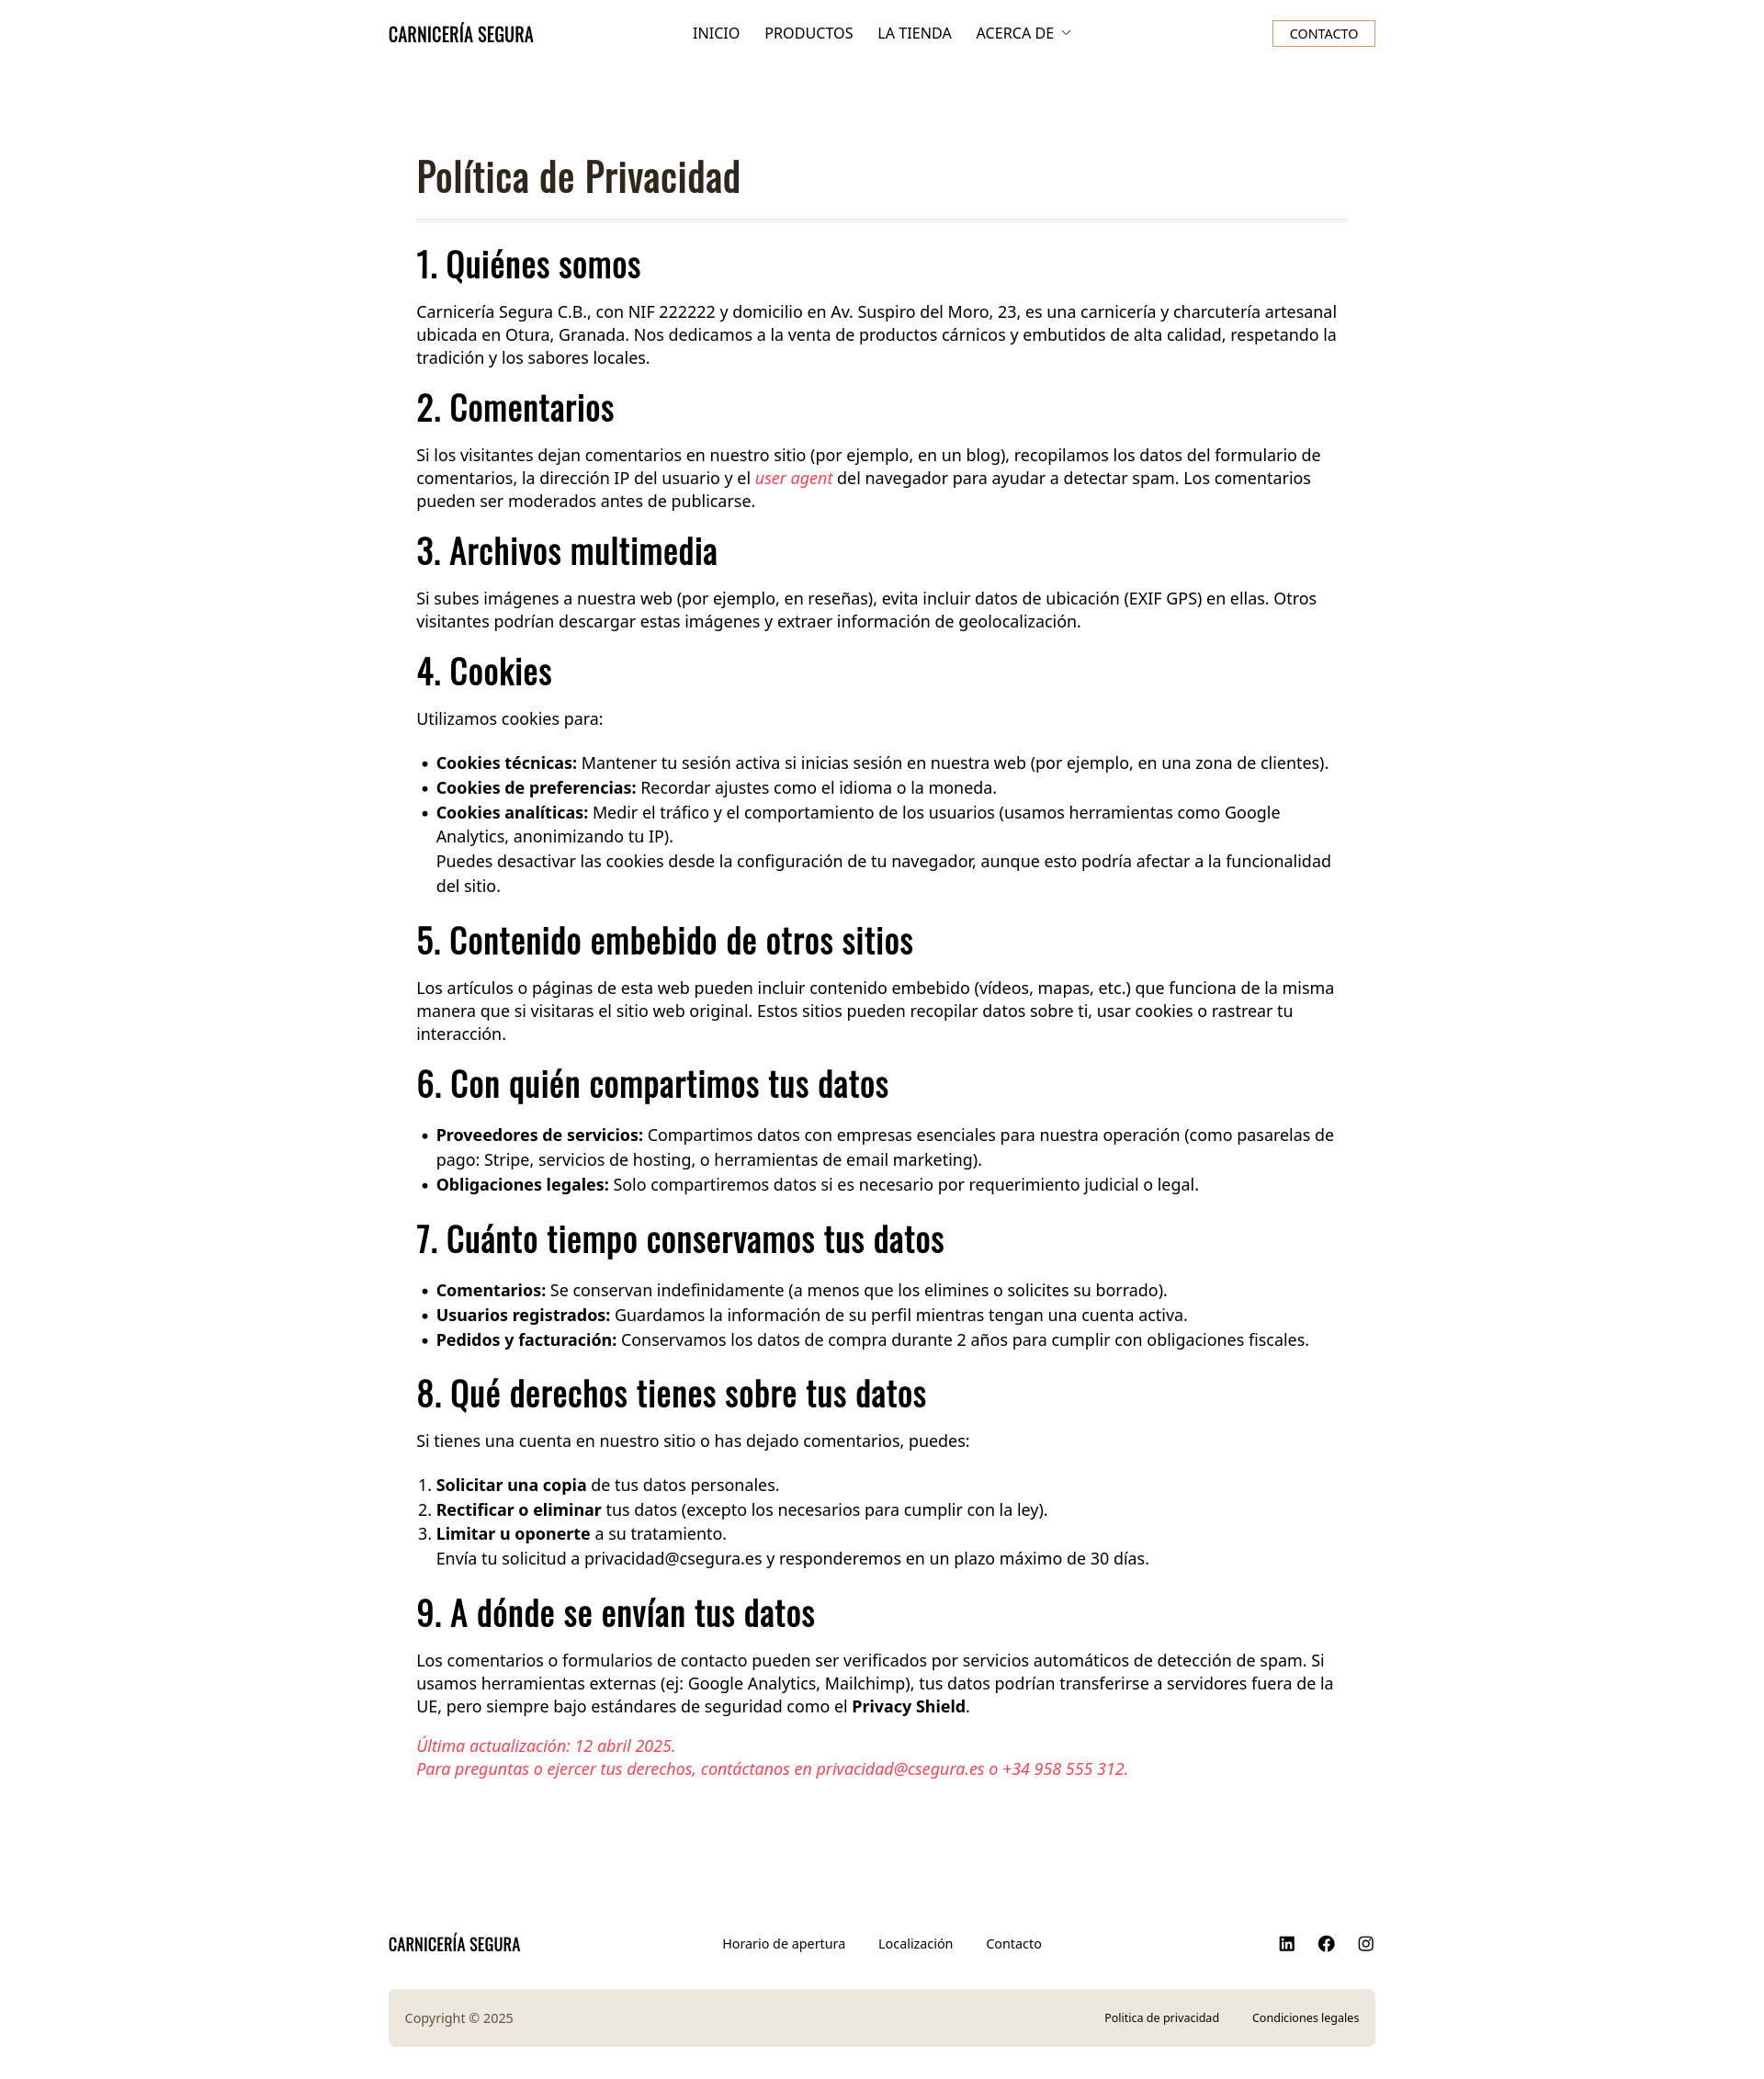
\includegraphics[width=1\textwidth]{images/privacy-policy.png}
    \caption{Política de privacidad}
\end{figure}

\begin{figure}[H]
    \centering
    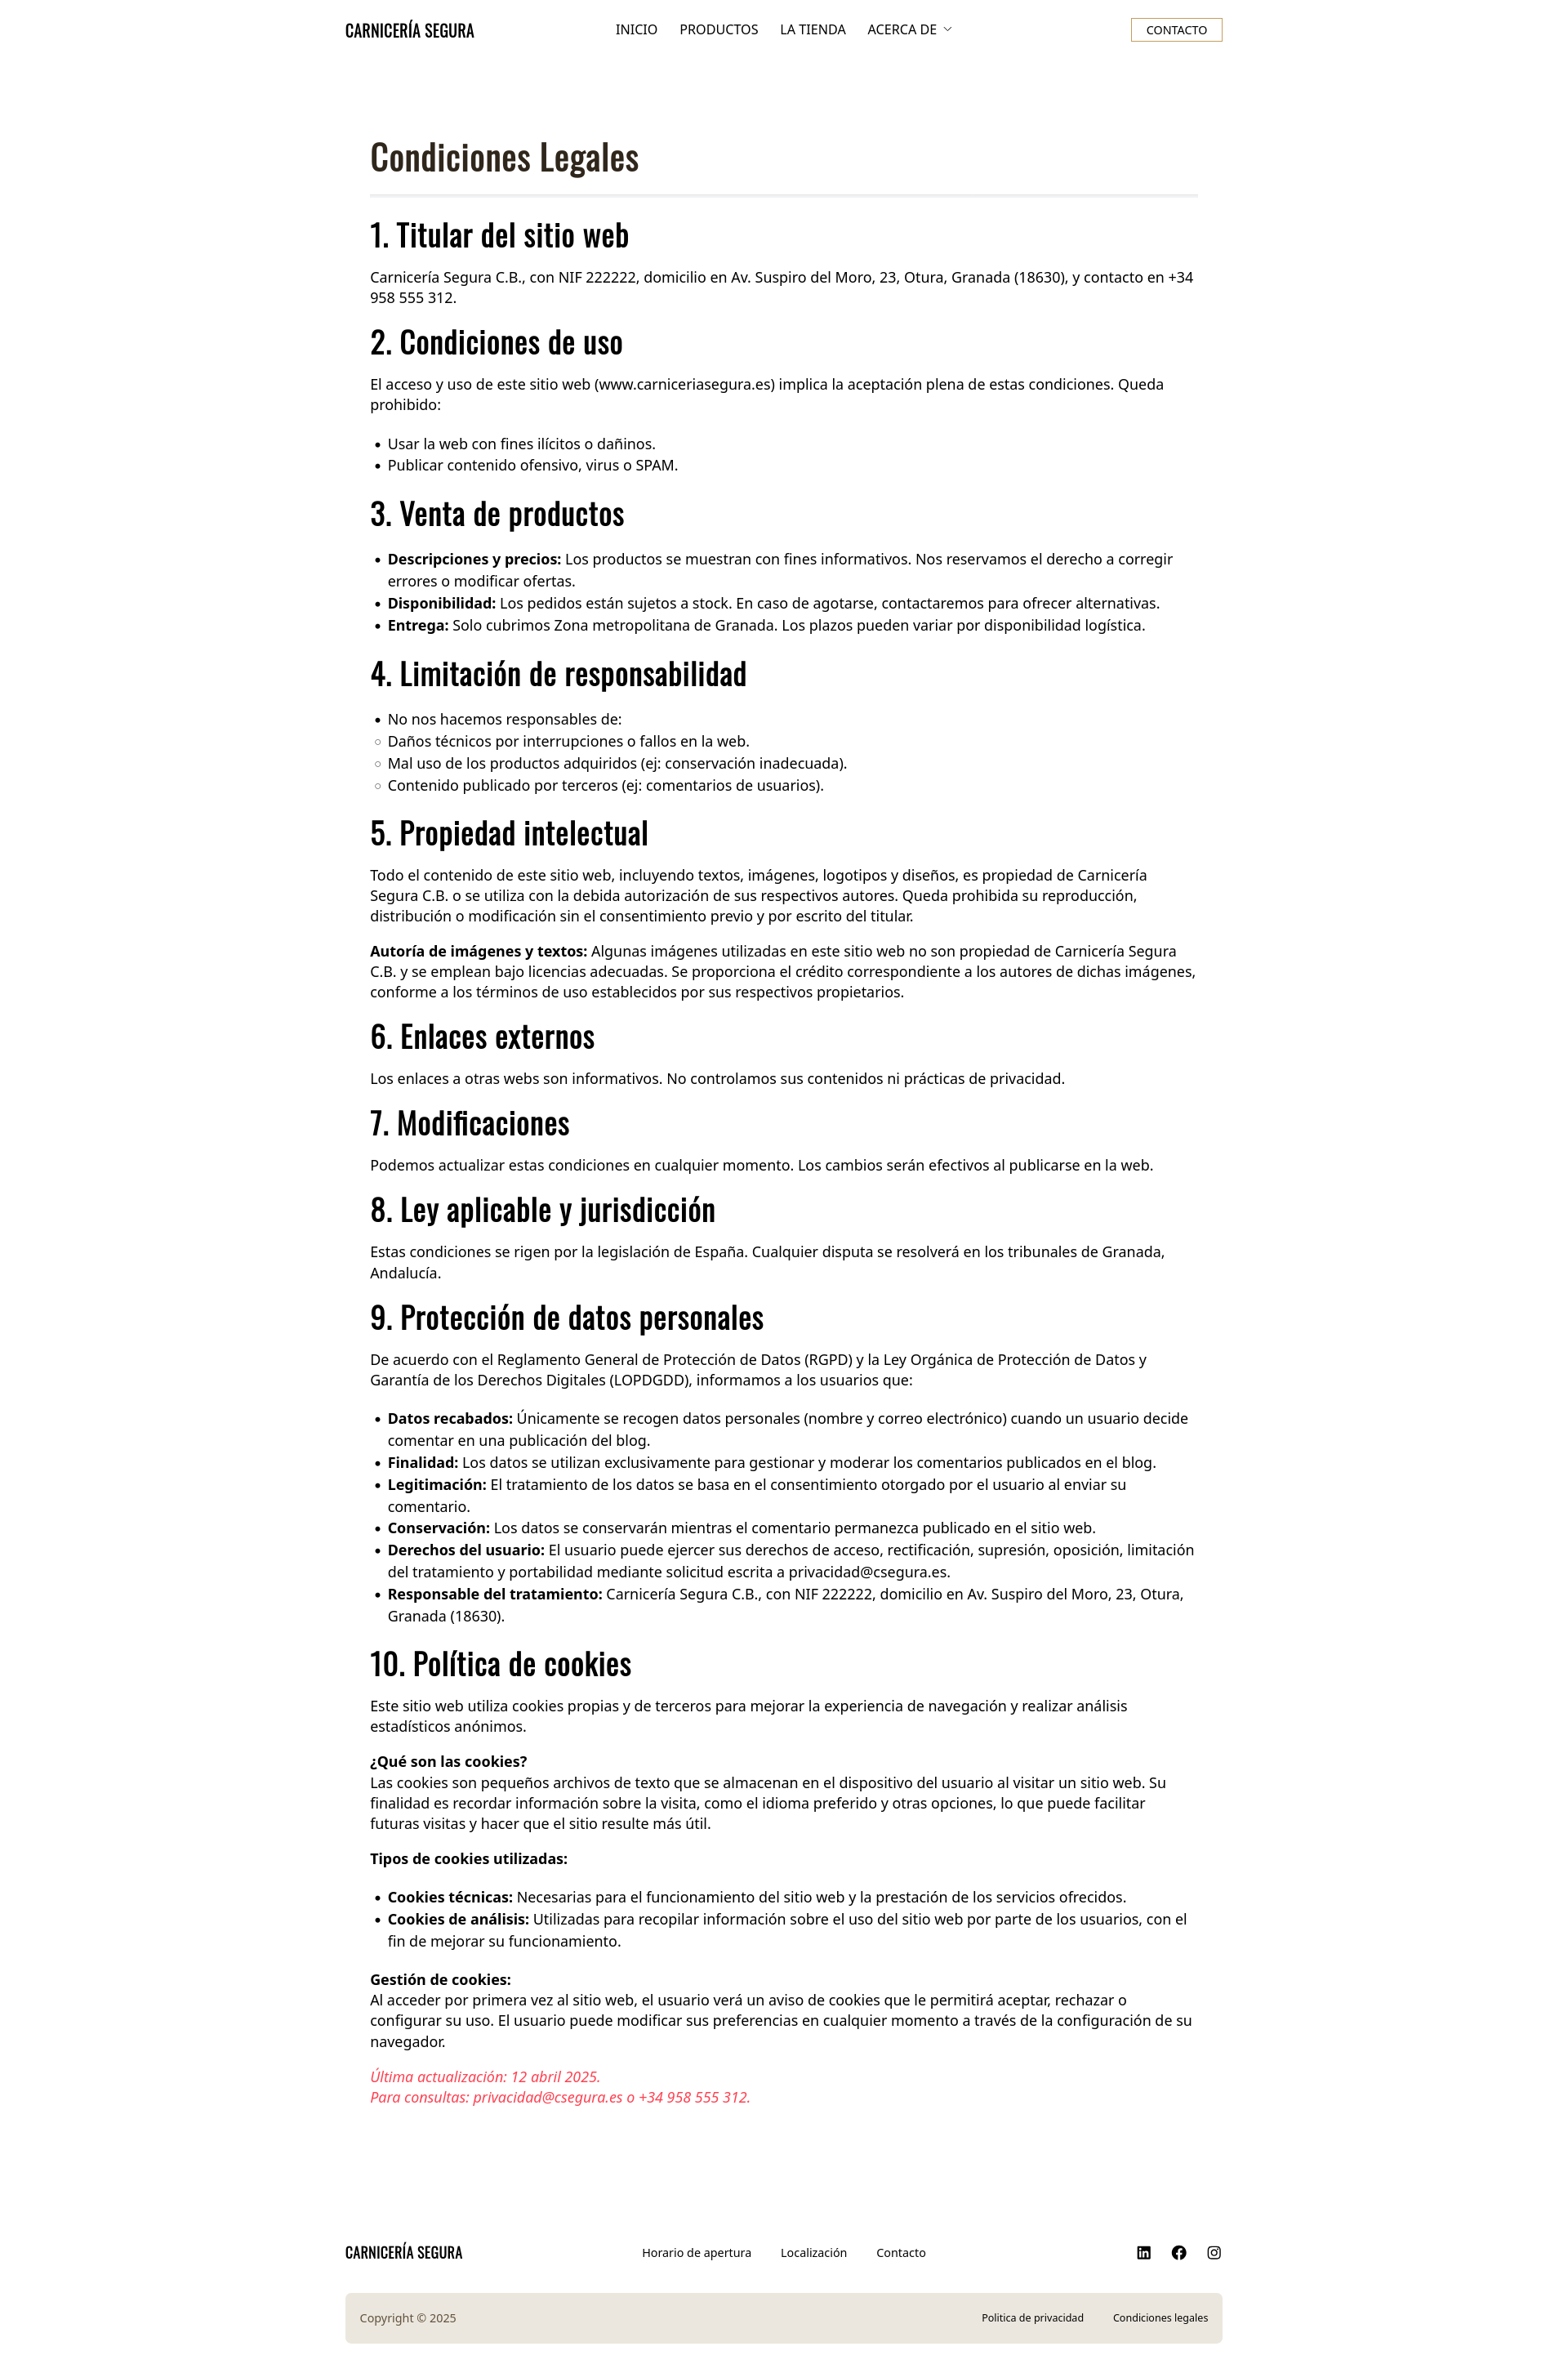
\includegraphics[width=1\textwidth]{images/legal-conditions.png}
    \caption{Aviso legal}
\end{figure}


\section{Backend}

\begin{figure}[H]
    \centering
    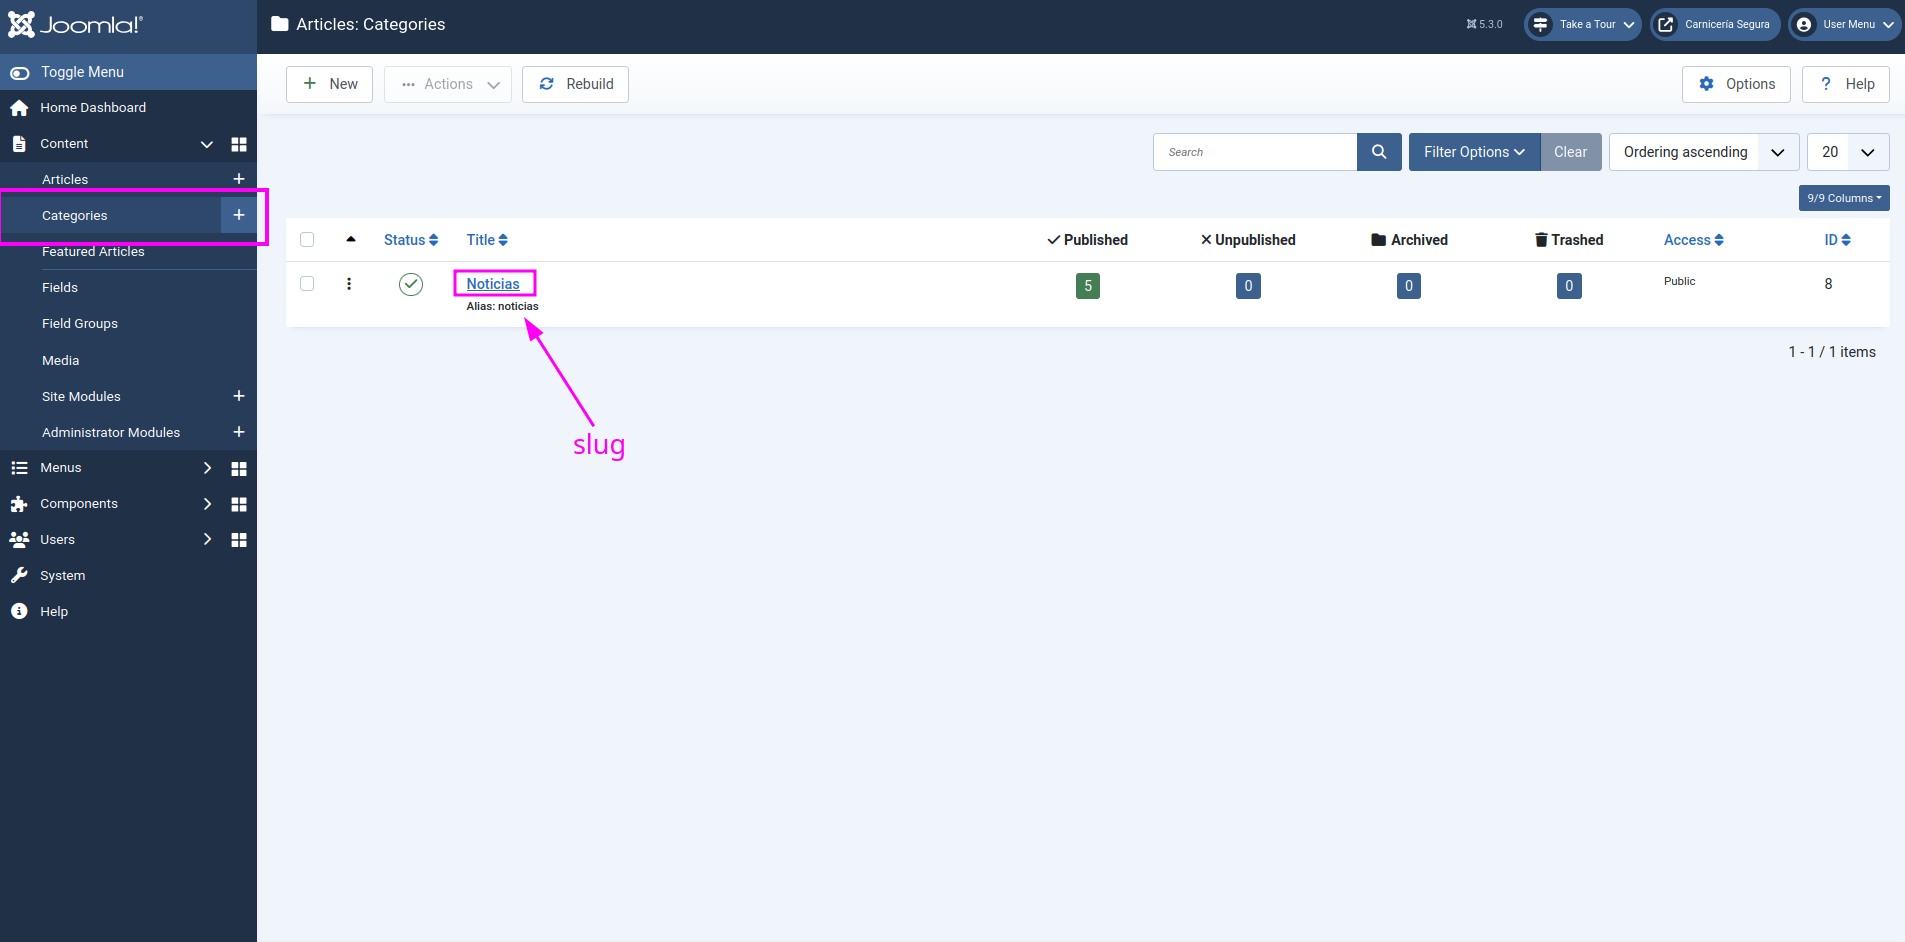
\includegraphics[width=0.9\textwidth]{images/backend-category.png}
    \captionsetup{width=0.85\textwidth}
    \caption{Categorías, similar a CPT en WordPress, pero funcionalidad por defecto en Joomla}
\end{figure}

\begin{figure}[H]
    \centering
    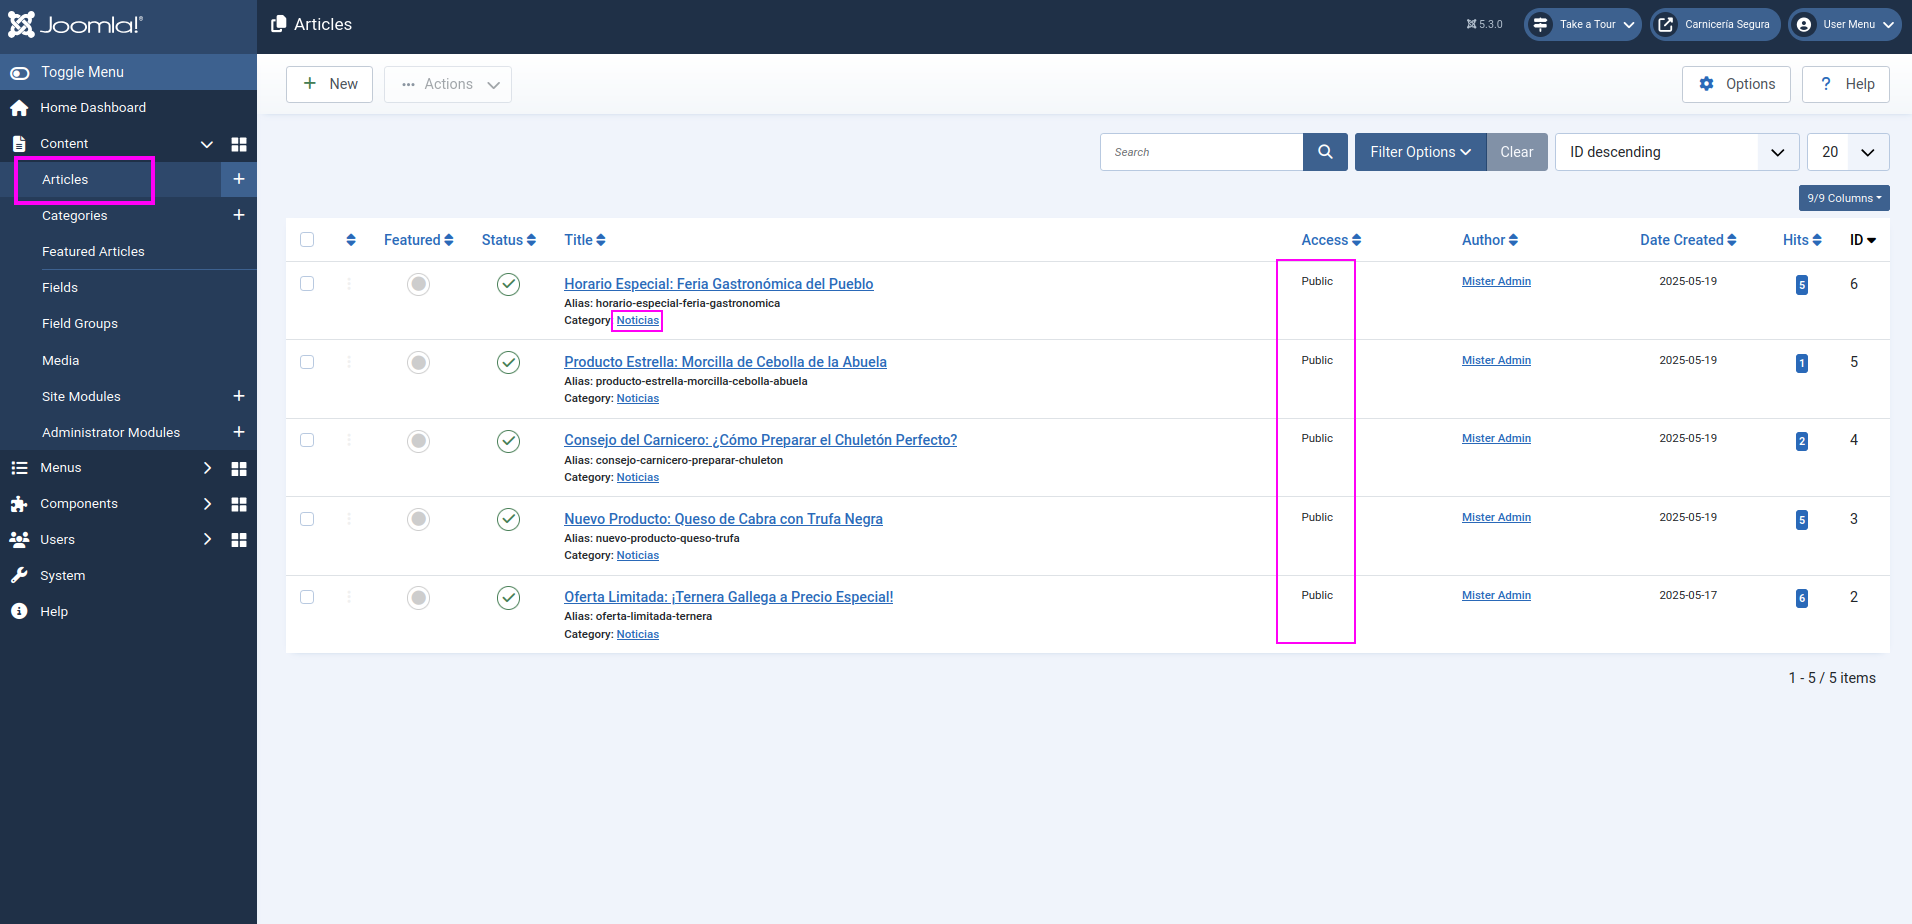
\includegraphics[width=0.9\textwidth]{images/backend-articles.png}
    \captionsetup{width=0.85\textwidth}
    \caption{Artículos, equivalente a entradas en WordPress. Cada artículo tiene su categoría}
\end{figure}

\begin{figure}[H]
    \centering
    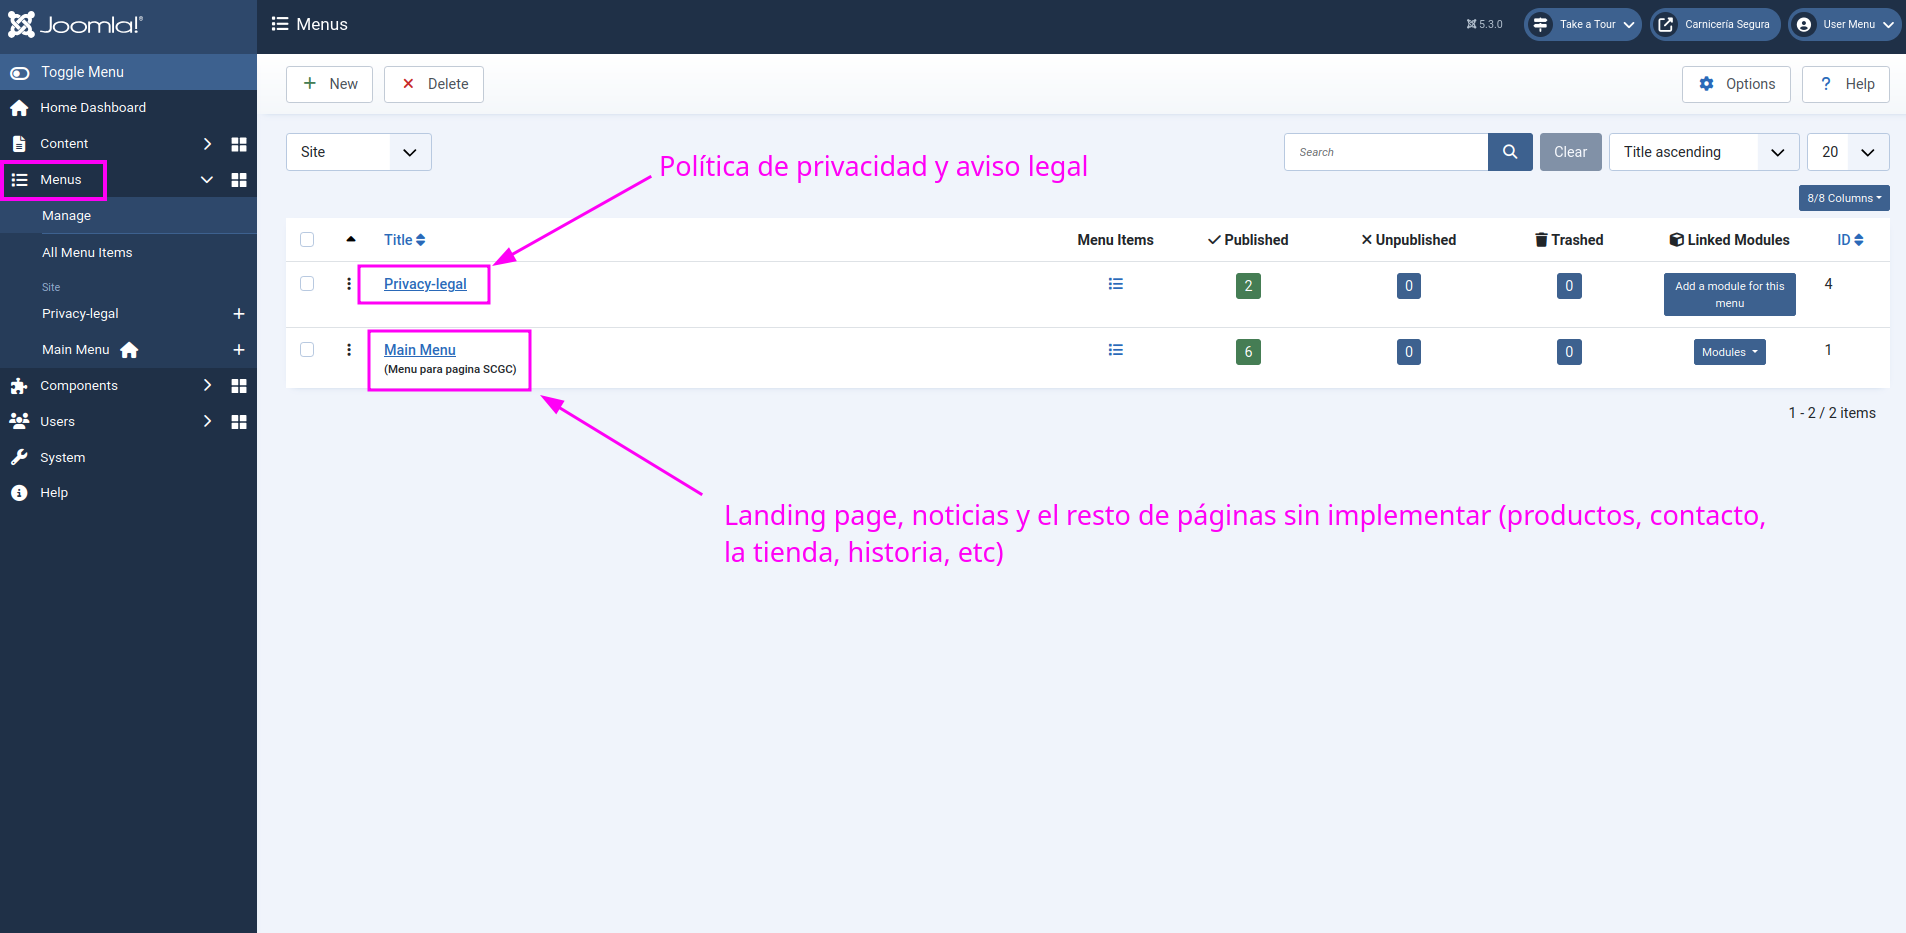
\includegraphics[width=0.9\textwidth]{images/backend-menus-overview.png}
    \captionsetup{width=0.85\textwidth}
    \caption{Overview de los menus, que agrupan lo equivalente a páginas}
\end{figure}

\begin{figure}[H]
    \centering
    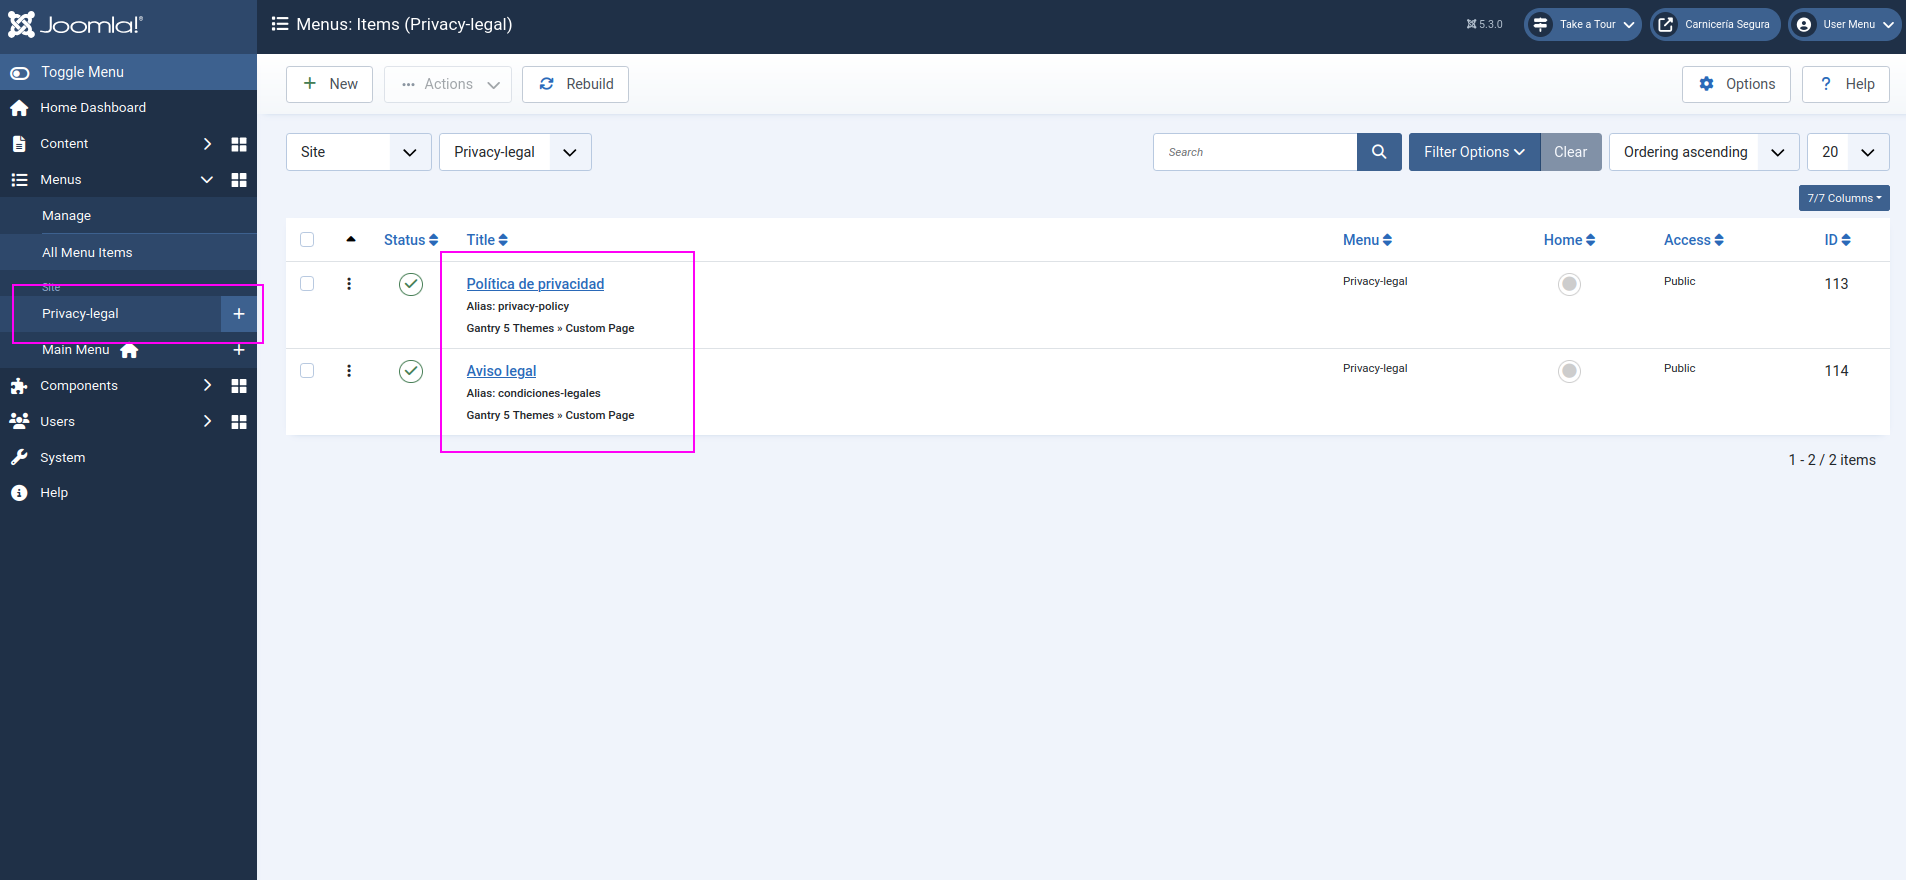
\includegraphics[width=0.9\textwidth]{images/backend-menu-privacy.png}
    \captionsetup{width=0.85\textwidth}
    \caption{Menú de privacidad y legal, con las dos páginas relevantes}
\end{figure}

\begin{figure}[H]
    \centering
    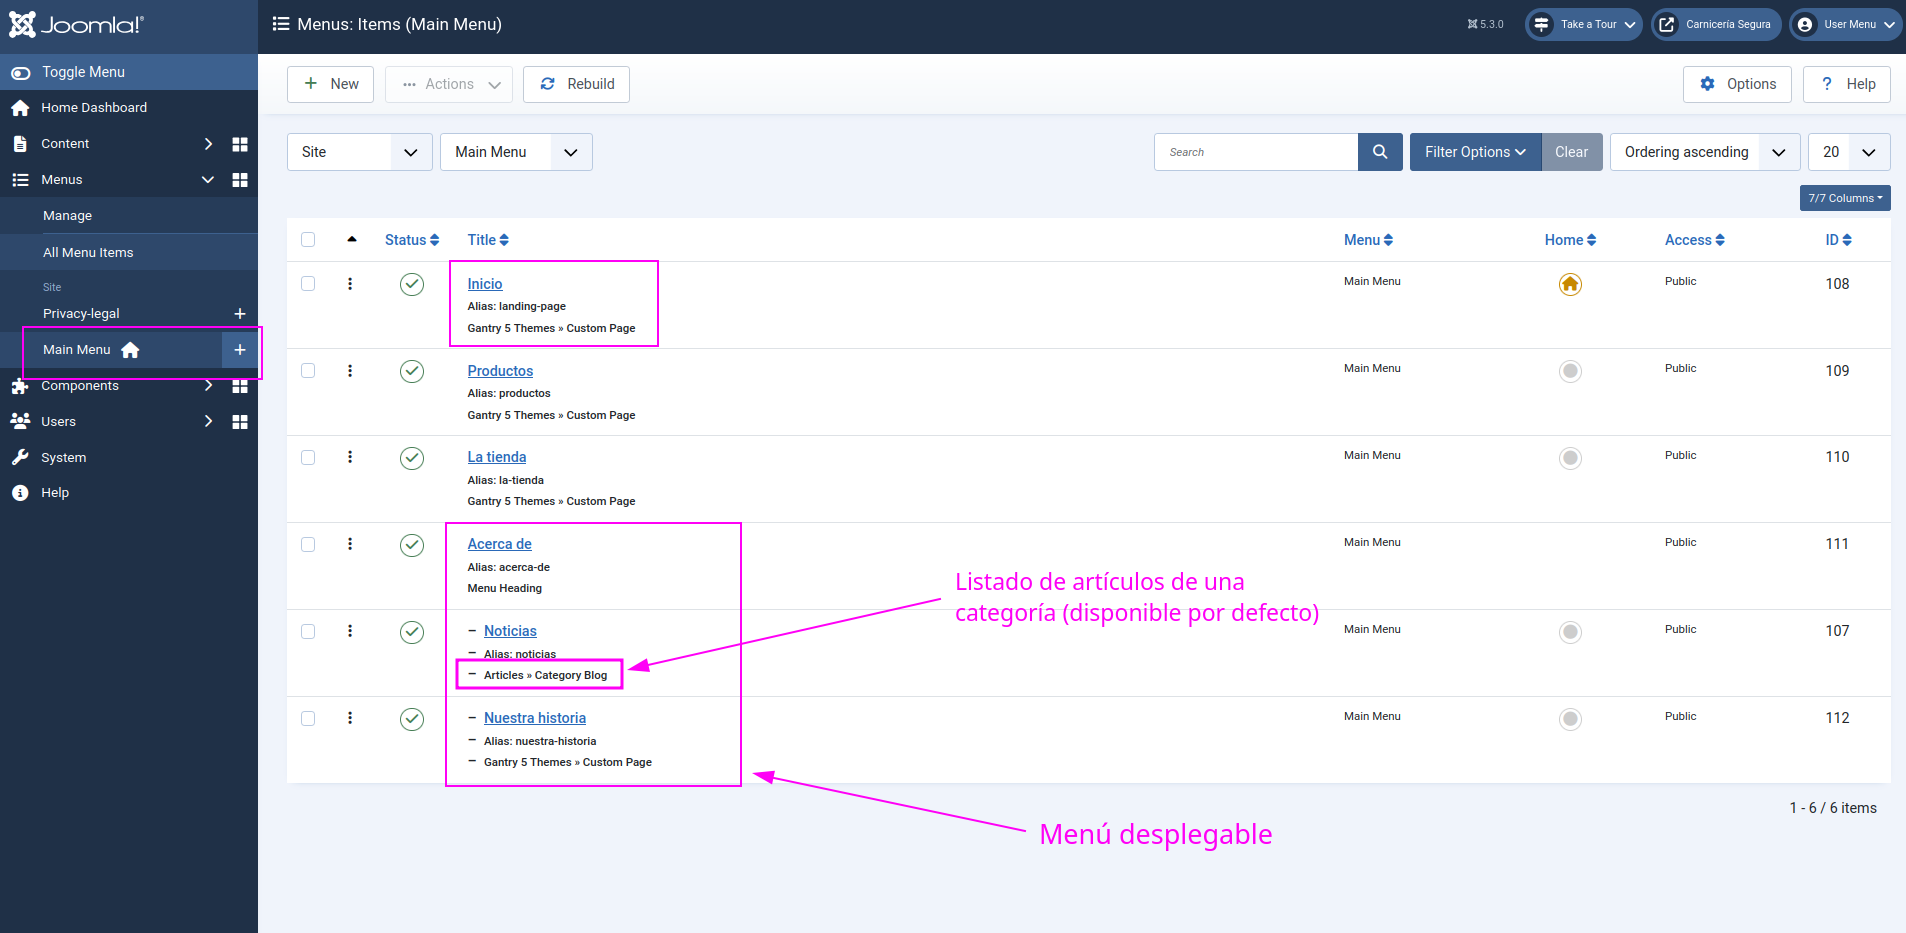
\includegraphics[width=0.9\textwidth]{images/backend-menu-main.png}
    \captionsetup{width=0.85\textwidth}
    \caption{Menú principal, asignado por defecto}
\end{figure}

\begin{figure}[H]
    \centering
    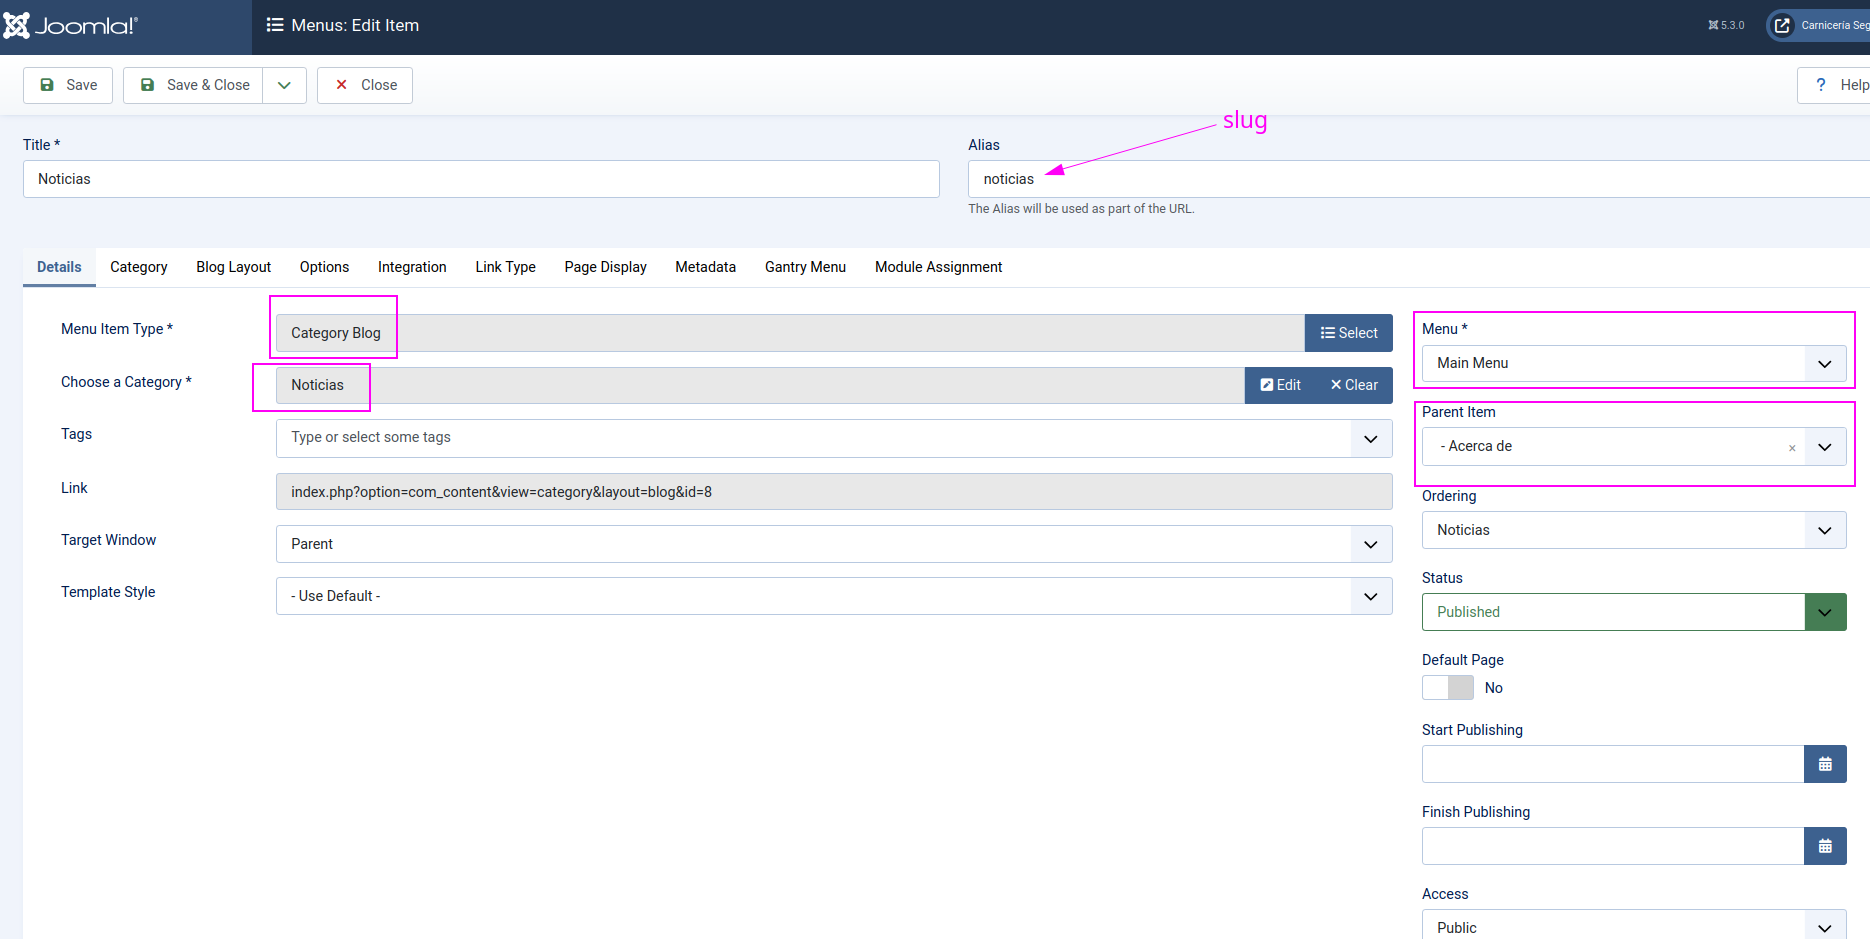
\includegraphics[width=0.9\textwidth]{images/backend-menu-news.png}
    \captionsetup{width=0.85\textwidth}
    \caption{Página para mostrar entradas de tipo \textit{Noticia}}
\end{figure}

\begin{figure}[H]
    \centering
    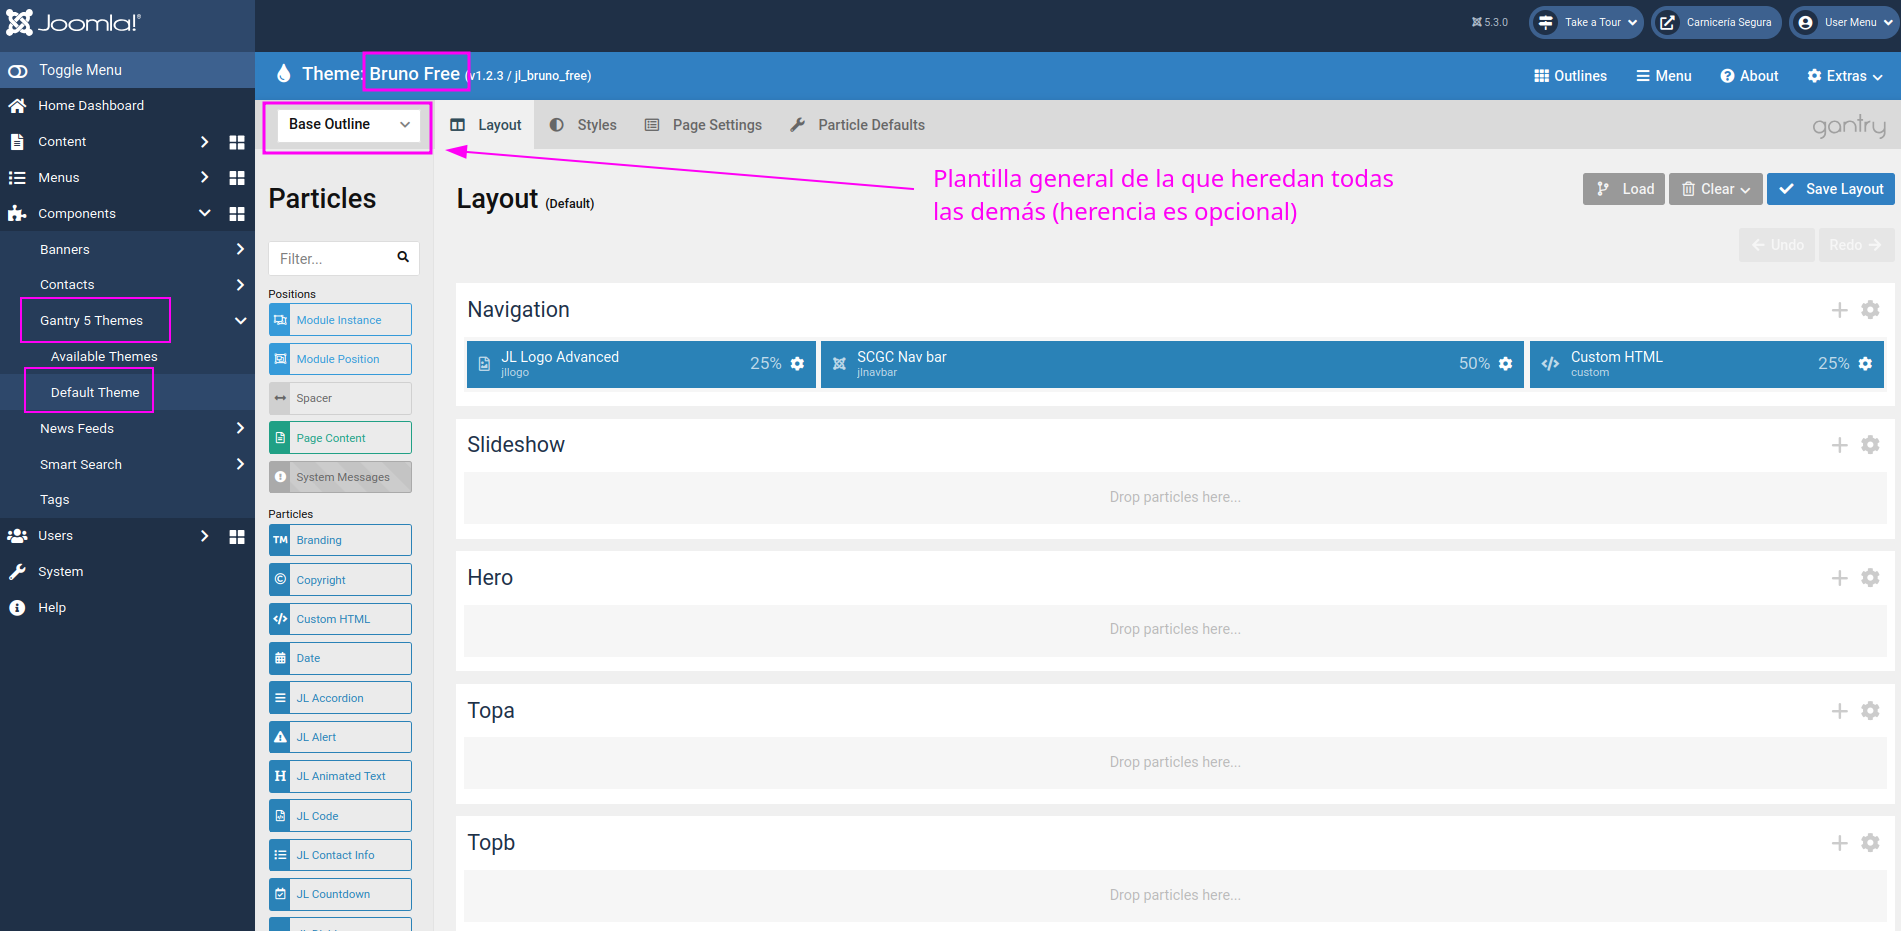
\includegraphics[width=0.9\textwidth]{images/backend-layout-base-outline.png}
    \captionsetup{width=0.85\textwidth}
    \caption{Editor de layouts de Gantry 5. Plantilla general que luego pueden heredar las otras páginas}
\end{figure}

\begin{figure}[H]
    \centering
    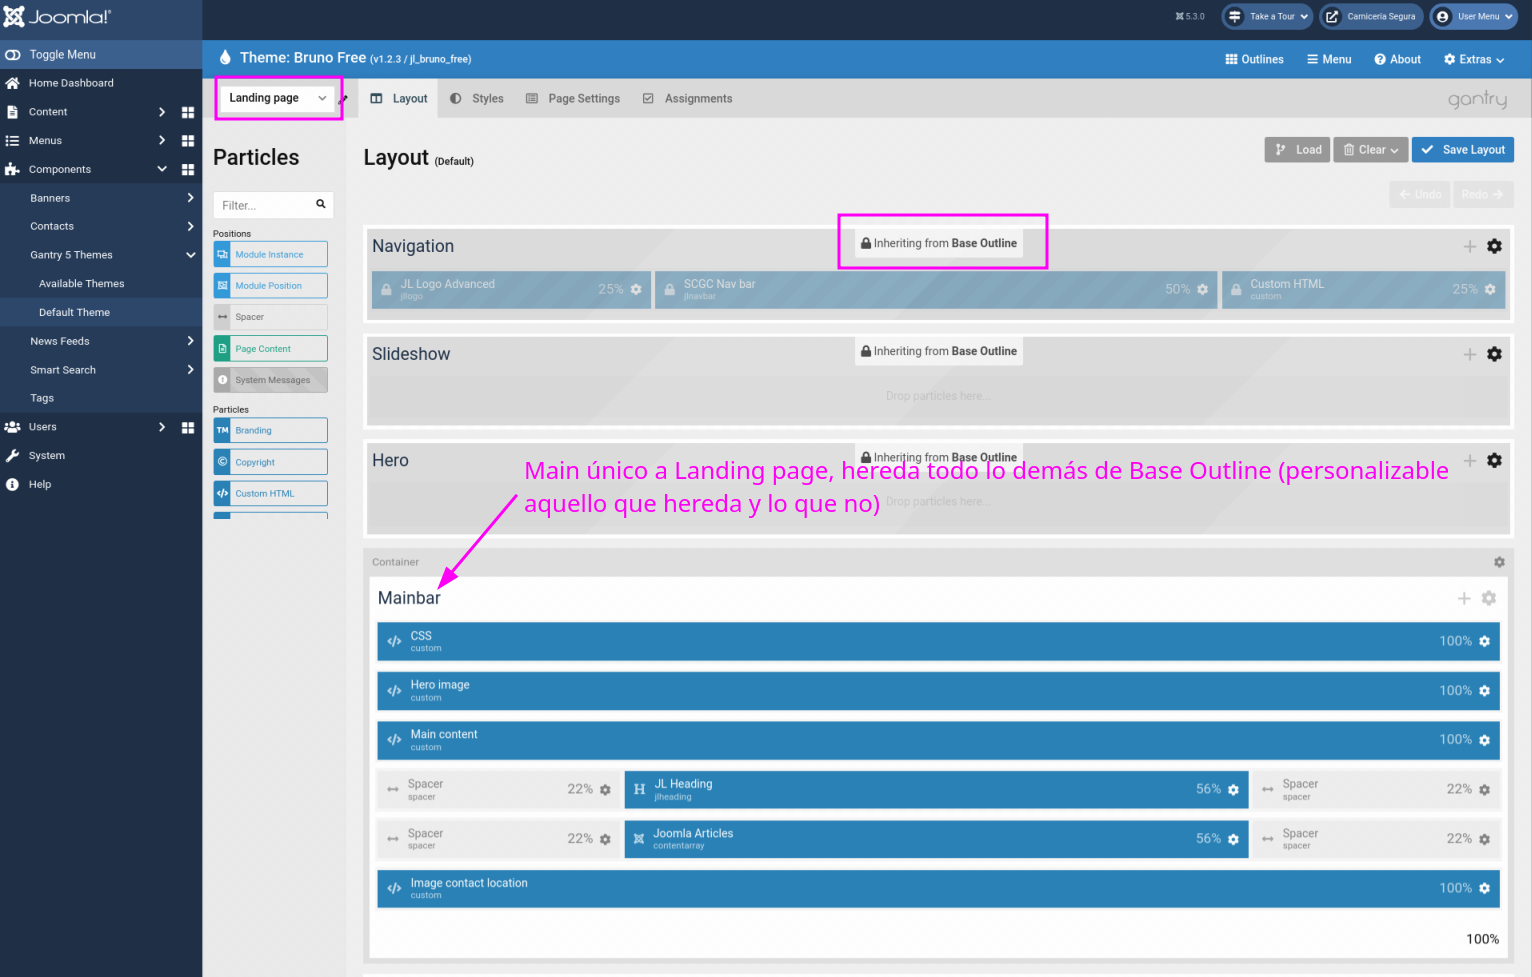
\includegraphics[width=0.9\textwidth]{images/backend-layout-landing-outline.png}
    \captionsetup{width=0.85\textwidth}
    \caption{Editor del layout de la landing page. Hereda todos los componentes menos el main}
\end{figure}


\section{Vídeo}

\href{https://drive.google.com/file/d/1qvQA09GjjR_p3fuuL1GLrYEpJQDwJftM/view?usp=sharing}{Enlace al vídeo de demostración}


\section{Anexo}

Debido a falta de tiempo se ha decidido saltar la implementación de los comentarios, es por eso que no aparecen en la landing page ni en las páginas de las noticias.



\end{document}
